\documentclass [12pt]{article}
\setlength{\textwidth}{6.25in}
\setlength{\textheight}{8.5in}
\setlength{\evensidemargin}{0in}
\setlength{\oddsidemargin}{0in}
\setlength{\topmargin}{-0.1in}
\setlength{\parskip}{.1in}  
\setlength{\parindent}{0.0in}  
\usepackage[left=3.5cm,right=2.5cm]{geometry}


\setcounter{secnumdepth}{4}
\setcounter{tocdepth}{4}
   
\usepackage{amsmath}
\usepackage{amssymb}
\usepackage{enumitem}
\usepackage{array}
\usepackage{caption} 
\numberwithin{equation}{section}
%\renewcommand{\theequation}{\thesection\arabic{equation}}

%NOTES

\usepackage{xargs}                      % Use more than one optional parameter in a new commands
\usepackage[pdftex,dvipsnames]{xcolor}  % Coloured text etc.
% 
\usepackage[colorinlistoftodos,prependcaption,textsize=tiny]{todonotes}
\newcommandx{\unsure}[2][1=]{\todo[linecolor=red,backgroundcolor=red!25,bordercolor=red,#1]{#2}}
\newcommandx{\change}[2][1=]{\todo[linecolor=blue,backgroundcolor=blue!25,bordercolor=blue,#1]{#2}}
\newcommandx{\info}[2][1=]{\todo[linecolor=OliveGreen,backgroundcolor=OliveGreen!25,bordercolor=OliveGreen,#1]{#2}}
\newcommandx{\improvement}[2][1=]{\todo[linecolor=Plum,backgroundcolor=Plum!25,bordercolor=Plum,#1]{#2}}
\newcommandx{\thiswillnotshow}[2][1=]{\todo[disable,#1]{#2}}


\definecolor{gold(metallic)}{rgb}{0.83, 0.69, 0.22}

\newcommand{\hwplotR}{\raisebox{2pt}{\tikz{\draw[red,solid,line width=0.9pt](0,0) -- (5mm,0);}}}
\newcommand{\hwplotY}{\raisebox{2pt}{\tikz{\draw[gold(metallic),solid,line width=0.9pt](0,0) -- (5mm,0);}}}
\newcommand{\hwplotG}{\raisebox{2pt}{\tikz{\draw[green,solid,line width=0.9pt](0,0) -- (5mm,0);}}}
\newcommand{\hwplotB}{\raisebox{2pt}{\tikz{\draw[blue,solid,line width=0.9pt](0,0) -- (5mm,0);}}}
\newcommand{\hwplotK}{\raisebox{2pt}{\tikz{\draw[black,dashed,line width=1.2pt](0,0) -- (5mm,0);}}}
\newcommand{\hwplotT}{\raisebox{2pt}{\tikz{\draw[black,solid,line width=1.2pt](0,0) -- (5mm,0);}}}


\usepackage{graphicx} % Used to insert images
\usepackage{adjustbox} % Used to constrain images to a maximum size 

\usepackage{bm}
%\usepackage[textsize=scriptsize]{todonotes}
\usepackage[hypcap]{caption}

\usepackage[hidelinks]{hyperref}




\usepackage{amsthm}
\newtheorem{prop}{Proposition}




%\usepackage{fontspec}
%\setmainfont{Times New Roman}
\setlength{\parskip}{.1in}  
\setlength{\parindent}{0.0in}  
\renewcommand{\baselinestretch}{1.5}
\renewcommand\contentsname{Contenido}
\renewcommand{\figurename}{Fig.}
\renewcommand{\listfigurename}{Lista de Figuras}
\renewcommand{\listtablename}{Lista de Tablas}
\usepackage{tikz}
%\usetikzlibrary{arrows,shapes,trees,..}
%\usepackage{pgflibraryarrows}
%\usepackage{pgflibrarysnakes}

\usepackage{longtable}
\usepackage[nottoc,numbib]{tocbibind}
\usepackage[round,sort]{natbib}
\renewcommand\refname{Referencias}

\newcommand{\myparagraph}[1]{\paragraph{#1}\mbox{}\\}
\newcommand{\PP}{\textit{\tiny P}}
\newcommand{\C}{\textit{\tiny C}}
\newcommand{\R}{\textit{\tiny R}}
\newcommand{\CR}{\textit{\tiny CR}}
\newcommand{\PC}{\textit{\tiny PC}}
\newcommand{\PR}{\textit{\tiny PR}}
\newcommand{\CP}{\textit{\tiny CP}}
\newcommand{\RC}{\textit{\tiny RC}}
\newcommand{\RP}{\textit{\tiny RP}}


%AMSMATH environment

\makeatletter
\newcommand{\mathleft}{\@fleqntrue}
\newcommand{\mathcenter}{\@fleqnfalse}
\makeatother

%Tikz===========================================

\usepackage{tikz,pgfplots}
\usetikzlibrary{arrows,calc}
\newenvironment{customlegend}[1][]{%
    \begingroup
    % inits/clears the lists (which might be populated from previous
    % axes):
    \csname pgfplots@init@cleared@structures\endcsname
    \pgfplotsset{#1}%
}{%
    % draws the legend:
    \csname pgfplots@createlegend\endcsname
    \endgroup
}%

% makes \addlegendimage available (typically only available within an
% axis environment):
\def\addlegendimage{\csname pgfplots@addlegendimage\endcsname}

%%--------------------------------

% definition to insert numbers
\pgfkeys{/pgfplots/number in legend/.style={%
        /pgfplots/legend image code/.code={%
            \node at (0.295,-0.0225){#1};
        },%
    },
}
%%===================================

\begin{document}
\setcounter{tocdepth}{3}
\tableofcontents
\listoffigures
\listoftables

\section{Abstract}
The body mass of a species due to its connection with metabolic rate and movement is a key trait which determine a lot of the species functionality, in this work we extend this line of thinking further by exploring how the body mass of the species which compose an intraguild predation module influence the maximum trophic position observed in the system and its structuration path (sequence of \textit{plausible} invasions) and coexistence zone. We derive relations that the mass of the interacting species must fulfill in order for an assembly path to be expressed and for the existence of a positive equilibrium, the form of this relationships is found to be insensitive to changes in basal productivity, foraging dimension and strategy; but they have a quantitative influence and in the case of the latter two, they could affect the qualitative behavior of some subparts of the relationship with respect to changes in the predator prey ratios present in the module. By its influence over this processes the combination of body masses affect the food chain length that could be found in the module. This results suggests promising conections between the assembly process of a comunity and the body mass of the species present in the regional pool and receptor comunity.

\keywords{Body mass, metabolism, intraguild predation, assembly, food chain}.

\subsection{INTRODUCCION}

Desde el descubrimiento y cuantificaci\'on de la relaci\'on existente entre la masa corporal de una especie y su tasa metab\'olica,lo que se denomin\'o \emph{kleiber's law} \citep{kleiber1961fire}, y la posterior sint\'esis de los registros emp\'iricos realizada porPeters \citep{peters1986ecological}; se suger\'ia una relaci\'on importante entre la masa corporal y la ecolog\'ia de las especies.Posteriormente Yodzis e Innes en su \emph{seminal paper, Body size and consumer resource dynamics}\citep{yodzis1992body} introdujeron estas ideas en los modelos depredador-presa,afectando particularmente la parametrizaci\'on de dichos modelos.Sin embargo formalizaci\'on de estas ideas bajo una teor\'ia se retras\'o hasta principios de este siglo bajo la denominada , \emph{Toer\'ia metab\'olica de la ecolog\'ia}(MTE), desarrollada entre otro por James Brown y Geoffrey West\citep{brown2004toward},a partir de ella se empez\'o a percibir de forma m\'as general la importancia del metabolismo, y por ende de la masa corporal, sobre distintos procesos ecol\'ogicos. Dada la caracter\'istica universal que tiene la relaci\'on entre la masa corporal y el metabolismo, la MTE y sus futuras extensiones tienen el potencial de convertirse en una teor\'ia que unifique las distintas \'areas de la ecolog\'ia.\\
En los \'ultimos a\~nos se han extendido los efectos de la masa a procesos comunitarios, en particular en el estudio de redes tr\'oficas, donde se ha sugerido particularmente que la masa de las especies interactuantes afectan la estabilidad, persistencia y funcionamiento de la red, debido a su influencia sobre la fuerza de interacci\'on entre especies y la velocidad de flujo de energ\'ia y masa a traves de ella. \citep{varios, citar luego}

Sin embargo a\'un no ha habido mucho \'enfasis en de que manera la masa corporal afecta el ensamblaje o estructuraci\'on de las comunidades ecolo\'ogicas.En este trabajo nos enfocamos en dicha direcci\'on y para ello analizamos el m\'odulo de tres especies denomidado \emph{Intraguild predation},el cual fue descrito en \cite{polis1989ecology} y el primera an\'alisis te\'orico desarrollado por \cite{holt1997theoretical}.Adem\'as, dada la conexi\'on existente entre el ensamblaje del m\'odulo y lo descrito por \cite{TP2007proximate} como \emph{mecanimos proximales de variaci\'on estructural de las cadenas tr\'oficas}, derivamos los efectos que la masa de las especies, y m\'as a\'un la raz\'on de masas presa-depredador, tienen sobre la longitud de las cadenas tr\'oficas. \\

La longitud de las cadenas tr\'oficas es una propiedad estructural importante de los ecosistemas ,que afecta distintas funciones ecol\'ogicas de \'este (e.g. reciclaje de nutrienes, patr\'on de efectos cascada), por lo cual  la observaci\'on de la variaci\'on de su longitud despert\'o y sigue despertando el inter\'es de muchos investigadores\citep{ulanowicz2014limits,borrelli2014there}, los cuales han tratado de determinar los factores que determinan esta longitud;si bien se han propuesto factores ambientales como posibles determinantes de la longitud: R\'egimen de disturbancias, Tama\~no del ecosistema y Nivel de productividad \citep{post2002long,takimoto2013environmental}; a\'un no se ha llegado a una conclusi\'on definitiva sobre los mecanismos que regulan esta longitud \citep{sterner1997enigma,takimoto2013environmental}. En los \'ultimos a\~nos se a pasado de determinar qu\'e factor es m\'as importante a determinar c\'omo los distintos factores interactuan entre s\'i y bajo que contexto son m\'as o menos importantes \citep{post2002long}.\\



\section{MARCO TEORICO}


\subsection{Modelos Matem\'aticos \emph{Depredador-Presa}}

El uso de modelos matem\'aticos para describir la din\'amica poblacional de un conjunto de especies que se relacionan mediante interacciones depredador-presa, se remonta a los trabajos de Lotka y Volterra\citep{gotelliprimer}, los cuales independientemente describieron los cambios en la abundancia poblacional de un depredador $C$ y una presa $R$ mediante el siguiente sistema de ecuaciones diferenciales : 

\begin{equation}\label{eq:LV}
\begin{aligned}
&\dot{R} = R(r - \alpha C)\\
&\dot{C} = C(e\alpha - q) 
\end{aligned}
\end{equation}

El sistema \eqref{eq:LV} es conocido como \emph{sistema de ecuaciones depredador-presa Lotka-Volterra} y se puede extender f\'acilmente a un sistema de $n$ especies identificadas con $\{1,2, \ldots ,n\}$ de la siguiente manera:
\begin{equation}\label{eq:LVGen}
\dot{X_i}  = X_i(b_i - d_i + \sum_{j}^n \alpha_{ij} X_j)
\end{equation}

Donde $X_i$ representa la abundancia en n\'umeros o biomasa de la especie $i$, $b_i$ la tasa intr\'inseca de producci\'on de masa(individuos), $d_i$ la tasa de p\'erdida de masa(individuos) y $\alpha_{ij}$ se puede interpretar como la p\'erdida(ganancia) de masa(individuos) debido a interacciones con las dem\'as especies presentes en el h\'abitat.

Por lo general se asume que :
\begin{itemize}
\item $\alpha_{ij}$ es una constante(la modificaci\'on $\alpha_{ij} = \alpha_{ij}(X)$ para una forma especf\'icia de la funci\'on da lugar a lo que se conoce como respuesta funcional tipo II  o tipo III).
\item $\alpha_{ii} < 0 $ si $X_i$ es un recurso basal, a diferencia de la formulaci\'on original en este caso se asume que existe \emph{denso dependencia directa} entre los individuos de una poblaci\'on de presas.
\item $\alpha_{ii} = 0 $ si $X_i$ es un depredador, es decir no existe \emph{denso dependencia directa} entre individuos de una poblaci\'on de depredadores, sin embargo la denso dependecia se da indirectamente a traves de la interacci\'on con los recursos..
\item $b_i = 0$ si $X_i$ es un depredador, ya que los depredadores no pueden subsistir en ausencia de presas.
\end{itemize}
Modelos como \eqref{eq:LVGen} son llamados \emph{modelos tipo Lotka-Volterra}.

El modelo depredador-presa \emph{Lotka-Volterra},pese a sus evidentes limitaciones,ha jugado(y sigue jugando) un papel importante en el desarrollo de la teor\'ia en ecolog\'ia y form\'o la base para el desarrollo de modelos que incorporan caracter\'isticas con mayor fundamento biol\'ogico. \\
Uno de los problemas que surge al momento de construir un modelo similar al de \eqref{eq:LVGen} es el como decidir \emph{a priori} el valor de los par\'ametros del modelo(e.g. $b_i , d_i$). Este problema se hace m\'as notorio conforme la dimensi\'on del modelo(i.e. n\'umero de ecuaciones en el sistema) crece \citep{yodzis1992body}.\\
Yodzis e Innes en su seminal paper \emph{Body size and Consumer-Resource dynamics}\citep{yodzis1992body} propusieron una forma para aligerar el problema.Ellos introdujeron lo que hoy en d\'ia se conoce como \emph{modelamiento bioenerg\'etico} el cual se basa en derivar los valores de los par\'ametros de las relaciones que existen entre ellos y la masa corporal, esta relaci\'on es generalmente de forma indirecta y se manifiesta debido a la influencia que tiene la masa sobre el metabolismo de las especies\citep{peters1986ecological}. A la fecha se han desarrollado diversos refinamientos a estas ideas, lo cual nos permite centrarnos en par\'ametros con mayor significado biol\'ogico.\citep{kiltie2000scaling,brown2004toward,savage2004predominance,pawar2012dimensionality,brose2010body}

\subsection{Ensamblaje}
En esta secci\'on definimos ciertos t\'erminos relacionados al proceso de ensamblaje de una comunidad. \\
Se denomina proceso de ensamblaje $E_A$ de una comunidad $A$ asociada a un h\'abitat $H$ al continuo de colonizaciones y extinciones de especies que se dan dentro de $H$, el conjunto de especies que \emph{potencialmente} puede colonizar a la comunidad $A$(i.e pueden por lo menos llegar a $H$) se denomina \emph{pool regional de especies}. 
\begin{equation}\label{eq:Assembly}
E_A := (A_0,H_0) \to (A_1,H_1) \to (A_2,H_2) \to \ldots
\end{equation}
En \eqref{eq:Assembly} cada cambio de $(A_i,H_i)$ a $(A_{i+1},H_{i+1})$ se da debido a un intento de colonizaci\'on sobre $(A_i,H_i)$,el cual puede tener uno de los tres siguientes desenlaces \citep{pawar2009community}: 
\begin{enumerate}
\item El invasor no puede invadir.
\item El invasor llega a invadir pero provoca extinciones en la comunidad receptora, pudiendo el mismo exintiguirse, esto es llamado \emph{invasi\'on inestable}.
\item El invasor llega a invadir y no provoca ninguna extinci\'on, esto es llamado \emph{invasi\'on estable}.
\end{enumerate}

De lo anterior se observa que la comunidad y h\'abitat f\'isico receptor juega un papel muy importante en el subsiguiente paso del proceso, adem\'as especificamos que cada estado $(A_i,H_i)$ puede estar en constante cambio,excepto por el n\'umero de especies, debido a la din\'amica inherente de las poblaciones de las especies presentes y por ende el tiempo entre distintas colonizaciones asu vez puede influenciar el desenlace de la colonizaci\'on debido a que la comunidad receptora puede estar en distintos estados(e.g. estado transiente $vs$ estado asint\'otico).\\

Sea $B = \{ (A_j,H_j) / j \in I, I \subseteq \mathbb{N}\}$ un conjunto de estados en $E_A$ , usando el formalismo definido en \eqref{eq:Assembly} decimos que la comunidad $A$ \emph{$\omega$-converge} a $B$ durante el ensamblaje si existe un $ m \in \mathbb{N}$ tal que $(A_i,H_i) \in B, i \geq m$. Sea $D$ el menor de dichos conjuntos. Decimos entonces que la comunidad $A$ \emph{converge} a $D$.

\subsubsection{Caminos de Ensamblaje}
Sea $\hat{A}$ un conjunto de especies con un set de interacciones $S$ , una secuencia de colonizaciones $E$ tal que el estado final es $(\hat{A},S)$ es llamado \emph{camino de ensamblaje} hacia $(\hat{A},S)$.

\subsection{ M\'odulo IGP}

En teor\'ia de redes tr\'oficas, se denomina \emph{community modules} a un conjunto peque\~no de especies que interact\'uan entre s\'i y cuyo patr\'on de interacci\'on ha sido encontrado en diversos ecosistemas(citar holt). Entre ellos el m\'odulo de \emph{depredaci\'on dentro del clan}(IGP por sus siglas en ingl\'es) fue descrito por primera vez por \cite{polis1989ecology} envuelve tres especies: un recurso basal, un depredador intermedio y un depredador tope.Ambos depredadores consumen al recurso y ademas el depredador intermedio es consumido por el depredador tope. Este sistema pese a tener solo $3$ especies incorpora diversos tipos de interacci\'on \emph{depredaci\'on, competencia aparente, competencia por explotaci\'on y mutualismo indirecto}. Esto se describe gr\'aficamente en la figura ~\ref{fig:IGP}
\begin{figure}[h]
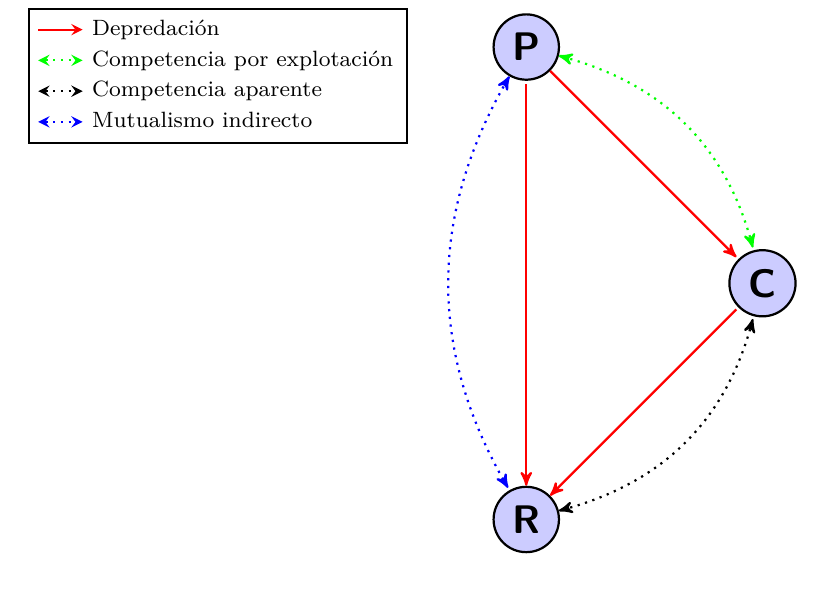
\begin{tikzpicture}[<->,>=stealth',shorten >=1pt,auto,
  thick,main node/.style={circle,fill=blue!20,draw,font=\sffamily\Large\bfseries}]


\node[main node] (R) at (0,-3){R};
\node[main node] (C) at (3,0) {C};
\node[main node] (P) at (0,3) {P};

 \path[every node/.style={font=\sffamily\small}]

(R) edge [<-,red] (C)
(R) edge [<-,red] (P)
(P) edge [->,red] (C)
(P) edge [bend right , dotted, blue] (R) 
(P) edge [bend left , dotted, green]  (C)
(R) edge [bend right ,dotted , black] (C);



\begin{customlegend}[legend cell align=left,
legend entries={ % <= in the following there are the entries
Depredaci\'on,
Competencia por explotaci\'on,
Competencia aparente, 
Mutualismo indirecto
},
legend style={at={(-1.5,3.5)},font=\footnotesize}] % <= to define position and font legend
% the following are the "images" and numbers in the legend
    \addlegendimage{-stealth,red}
    \addlegendimage{stealth-stealth,dotted,green}
    \addlegendimage{stealth-stealth,dotted,black}
    \addlegendimage{stealth-stealth,dotted,blue}
    
\end{customlegend}

\end{tikzpicture}

\caption{M\'odulo \textbf{IGP}}
\label{fig:IGP}
\end{figure}

Adem\'as este sistema es el menor(en el sentido de n\'umero de especies) en el cual podemos encontrar 2 \emph{caminos de ensamblaje}.
\begin{figure}[h]
\begin{center}
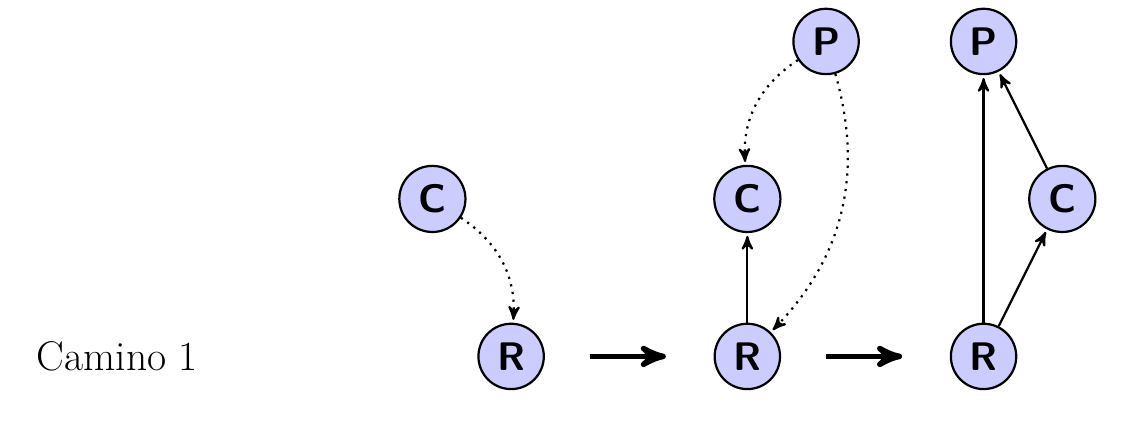
\begin{tikzpicture}[->,>=stealth',shorten >=1pt,auto,
  thick,main node/.style={circle,fill=blue!20,draw,font=\sffamily\Large\bfseries}]

\node[main node](R1) at (1,0) { R};
\node[main node](C1) at (0,2) {C};
\node[main node](C2) at  (4,2){C};
\node[main node](R2) at ($(R1) + (3,0)$) {R};
\node[main node](P1) at (5,4){P};
\node[main node](R3) at ($(R2) + (3,0)$){R};
\node[main node](C3) at ($(R3) + (1,2)$){C};
\node[main node](P3) at ($(R3) + (0,4)$){P};
\node[font = \fontsize{15}{15}\selectfont](A1) at (-4,0) {Camino 1};

\path
(C1) edge[bend left,dotted] (R1)
($(R1)+(1.0,0)$) edge[line width = 2]  ($(R1)+ (2,0)$)
(R2) edge (C2)
(P1) edge[bend right,dotted] (C2)
(P1) edge[bend left,dotted] (R2)
($(R2) + (1.0,0)$) edge[line width  = 2] ($(R2) + (2,0)$)
(R3) edge (C3)
(R3) edge (P3)
(C3) edge (P3);
\end{tikzpicture}
$\left. \right.$\\
$\left. \right.$\\

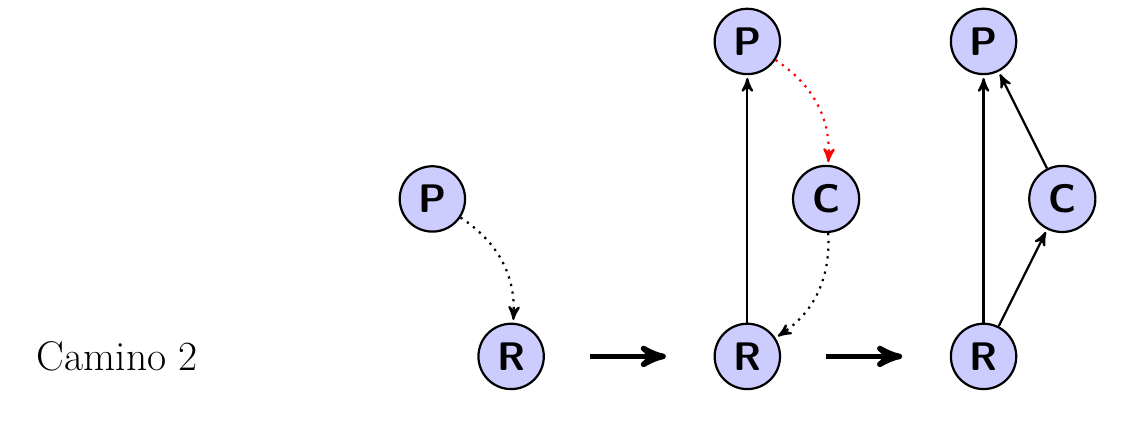
\begin{tikzpicture}[->,>=stealth',shorten >=1pt,auto,
  thick,main node/.style={circle,fill=blue!20,draw,font=\sffamily\Large\bfseries}]

\node[main node](R1) at (1,0) { R};
\node[main node](P1) at (0,2) {P};
\node[main node](P2) at  (4,4){P};
\node[main node](R2) at ($(R1) + (3,0)$) {R};
\node[main node](C1) at (5,2){C};
\node[main node](R3) at ($(R2) + (3,0)$){R};
\node[main node](C3) at ($(R3) + (1,2)$){C};
\node[main node](P3) at ($(R3) + (0,4)$){P};
\node[font = \fontsize{15}{15}\selectfont](A1) at (-4,0) {Camino 2};

\path
(P1) edge[bend left,dotted] (R1)
($(R1)+(1.0,0)$) edge[line width = 2]  ($(R1)+ (2,0)$)
(R2) edge (P2)
(C1) edge[bend left,dotted] (R2)
(P2) edge[bend left,dotted,red] (C1)
($(R2) + (1.0,0)$) edge[line width  = 2] ($(R2) + (2,0)$)
(R3) edge (C3)
(R3) edge (P3)
(C3) edge (P3);

\end{tikzpicture}
\end{center}

\caption{\emph{Caminos de ensamblaje} para el m\'odulo \textbf{IGP}}
\label{fig:IGPAssembly}
\end{figure}
Numerosos ejemplos son citados en \cite{polis1989ecology}, algunos de los cuales se presentan en la siguiente tabla:
\improvement{HACER LA TABLA!}

\subsection{Distribuci\'on de Masas}
Una distribuci\'on de masas en una comunidad $C$ es la imagen de una funci\'on  $f : C \to \mathbb{R}$ donde a cada conjunto de individuos de una especie $S$ se le asocia la masa promedio $m_S$ encontrada en $S$. Una distribuci\'on de masas proveniente de una recolecci\'on emp\'irica se representa gr\'aficamente mediante histogramas. \\
Generalmente la forma de la distribuci\'on se considera una caracter\'istica de la comunidad, y se ha demostrado que influencia la distribuci\'on de autovalores y otras propiedades din\'amicas de ella.\\

En el m\'odulo IGP dado que solo esta compuesto de tres especies podemos describir la distribuci\'on de las masas presentes en el m\'odulo mediante las relaciones que existen entres las masas de las tres especies y distinguir estos 6 tipos de comunidades :
\begin{enumerate}
  \item $m_P > m_C > m_R$
  \item $m_P > m_R > m_C$
  \item $m_R > m_C > m_P$
  \item $m_R > m_P > m_C$
  \item $m_C > m_P > m_R$
  \item $m_C > m_R > m_P$
\end{enumerate}

Estas relaciones entre masas son equivalentes a relaciones entre las razones de masas presentes en el m\'odulo. 
Definimos :
\begin{equation}\label{eq:SR}
  \begin{aligned}
    &k_{\RC} \equiv \frac{m_R}{m_C}\\
    &k_{\CP} \equiv \frac{m_C}{m_P}\\
    &k_{\RP} \equiv \frac{m_R}{m_P} = k_{\RC} k_{\CP}
  \end{aligned}
\end{equation}

Podemos designar cada comunidad por su particular relaci\'on de masas :
\begin{enumerate}[label=(\alph*)]
\item $\mathbf{C}_1$ sss $k_{\RC} < 1 , k_{\RP} < 1 ,k_{\CP} < 1$
\item $\mathbf{C}_2$ sss $k_{\RC} > 1 , k_{\RP} < 1 ,k_{\CP} < 1$
\item $\mathbf{C}_3$ sss $k_{\RC} > 1 , k_{\RP} > 1 ,k_{\CP} < 1$
\item $\mathbf{C}_4$ sss $k_{\RC} > 1 , k_{\RP} > 1 ,k_{\CP} > 1$
\item $\mathbf{C}_5$ sss $k_{\RC} < 1 , k_{\RP} > 1 ,k_{\CP} > 1$
\item $\mathbf{C}_6$ sss $k_{\RC} < 1 , k_{\RP} < 1 ,k_{\CP} > 1$
\end{enumerate}

Bajo este criterio podemos seccionar el espacio $k_{\CP} \times k_{\RC}$ en 6 zonas. Esto se represta gr\'aficamente en la figura ~\ref{fig:ZonasSR}

\begin{figure}[h!]
  \centering
  \begin{tikzpicture}[<->,>=stealth',shorten >=0.1pt,auto,
  thick,main node/.style={circle,fill=blue!20,draw,font=\sffamily\Large\bfseries}]


\node (fig1) at (-3,-5)
       {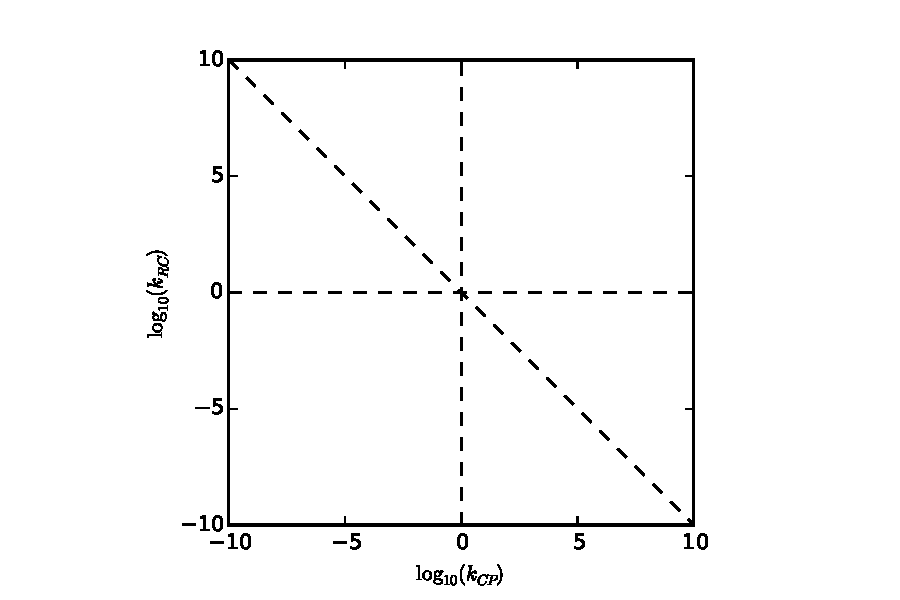
\includegraphics[scale=0.8]{C:/Users/Carlos/Documents/Tesis-IGP/code/Theory/ZonesSR.pdf}};

\node[circle,fill= blue!20,draw, minimum size=0.6cm,inner sep= 0] (R) at (-5.5,-4.5){R};
\node[circle,fill=blue!20,draw,minimum size=0.3cm, inner sep = 0] (C) at (-4.5,-3.8) {C};
\node[circle,fill=blue!20,draw,minimum size=1.cm,inner sep = 0](P) at (-5.5,-3.) {P};

 \path[every node/.style={font=\sffamily\small}]

(R) edge [<-,red] (C)
(R) edge [<-,red] (P)
(P) edge [->,red] (C);


\node[circle,fill= blue!20,draw, minimum size=0.3cm,inner sep= 0] (R) at (-4.5,-7.8){R};
\node[circle,fill=blue!20,draw,minimum size=0.6cm, inner sep = 0] (C) at (-3.5,-6.7) {C};
\node[circle,fill=blue!20,draw,minimum size=1.cm,inner sep = 0](P) at (-4.5,-5.6) {P};

 \path[every node/.style={font=\sffamily\small}]

(R) edge [<-,red] (C)
(R) edge [<-,red] (P)
(P) edge [->,red] (C);


\node[circle,fill= blue!20,draw, minimum size=1.cm,inner sep= 0] (R) at (-3.4,-3.6){R};
\node[circle,fill=blue!20,draw,minimum size=0.3cm, inner sep = 0] (C) at (-4.3,-2.6) {C};
\node[circle,fill=blue!20,draw,minimum size=0.6cm,inner sep = 0](P) at (-3.4,-2.1) {P};

 \path[every node/.style={font=\sffamily\small}]

(R) edge [<-,red] (C)
(R) edge [<-,red] (P)
(P) edge [->,red] (C);



\node[circle,fill= blue!20,draw, minimum size=1.cm,inner sep= 0] (R) at (-1.5,-4.1){R};
\node[circle,fill=blue!20,draw,minimum size=0.6cm, inner sep = 0] (C) at (-0.3,-3) {C};
\node[circle,fill=blue!20,draw,minimum size=0.3cm,inner sep = 0](P) at (-1.5,-2.1) {P};

 \path[every node/.style={font=\sffamily\small}]

(R) edge [<-,red] (C)
(R) edge [<-,red] (P)
(P) edge [->,red] (C);


\node[circle,fill= blue!20,draw, minimum size=0.6cm,inner sep= 0] (R) at (-0.1,-7){R};
\node[circle,fill=blue!20,draw,minimum size=1.0cm, inner sep = 0] (C) at (-1,-5.9) {C};
\node[circle,fill=blue!20,draw,minimum size=0.3cm,inner sep = 0](P) at (-0.1,-5.2) {P};

 \path[every node/.style={font=\sffamily\small}]

(R) edge [<-,red] (C)
(R) edge [<-,red] (P)
(P) edge [->,red] (C);


\node[circle,fill= blue!20,draw, minimum size=0.3cm,inner sep= 0] (R) at (-2.55,-7.8){R};
\node[circle,fill=blue!20,draw,minimum size=1.cm, inner sep = 0] (C) at (-1.8,-6.7) {C};
\node[circle,fill=blue!20,draw,minimum size=0.6cm,inner sep = 0](P) at (-2.55,-5.7) {P};

 \path[every node/.style={font=\sffamily\small}]

(R) edge [<-,red] (C)
(R) edge [<-,red] (P)
(P) edge [->,red] (C);


   
\end{tikzpicture}

  \caption{Divisi\'on del espacio $k_{\CP} \times k_{\RC}$ en funci\'on ah las relaciones de orden existentes entre las masas de las tres especies.}
\label{fig:ZonasSR}
\end{figure}
  








\section{OBJETIVOS GENERALES Y ESPEC\'IFICOS}
\subsection{Objetivo General}
Desarrollar un mejor entendimiento de los mecanismos que regulan la longitud de las cadenas tr\'oficas.
\subsection{Objetivos Espec\'ificos}
\begin{itemize}
\item Derivar condiciones necesarias y suficientes para la expresi\'on de los mecanismos responsables de la variaci\'on en la longitud de las cadenas tr\'oficas(e.g. inserci\'on, adici\'on y  grado de omnivor\'ismo); dependientes de la raz\'on de masas depredador-presa presentes en la comunidad.
\item Evaluar la influencia de factores como la dimensi\'on del ecosistema, la estrategia de forrajeo de los depredadores presentes y el nivel de productividad basal del ecosistema, sobre dichas condiciones.
\end{itemize}

\section{HIPOTESIS}
\begin{itemize}
\item[$H_{o1}:$] La longitud de las cadenas tr\'oficas es invariante respecto a cambios en los valores de la raz\'on de masas presa-depredador presentes en la comunidad.
\item[$H_{11}:$] La longitud de las cadenas tr\'oficas es dependiente de los valores de la raz\'on de masas presa-depredador presentes, debido a las limitaciones que estos imponen sobre los mecanismos de inserci\'on, adici\'on y omnivorismo.

\item[$H_{o2}:$] Las limitaciones impuestas sobre la longitud de las cadenas tr\'oficas por los  valores de la raz\'on de masas presa-depredador presentes en la comunidad es independiente de la dimensi\'on del ecosistema, la estrategia de forrajeo de los depredadores presentes y el nivel de productividad basal del ambiente.
\item[$H_{12}:$] La dimensi\'on del ecosistema, la estrategia de forrajeo de los depredadores presentes y el nivel de productividad basal del ambiente influencian las limitaciones que impone sobre la longitud de las cadenas tr\'oficas los valores de la raz\'on de masas presa-depredador presentes en la comunidad,debido a que modulan sus relaciones con los mecanimos de inserci\'on,adici\'on y omnivorismo.

\end{itemize}


\section{METODOLOGIA}

\subsection{Modelaci\'on matem\'atica}

Tomando como base el m\'odulo de tres especies \emph{depredaci\'on intragremial}-(descrito en \citealt{polis1989ecology,polis1992intraguild}),usamos un modelo matem\'atico \citep{holt1997theoretical} para describir las interacciones entre las especies componentes (recurso, consumidor intermedio(IG presa) y depredador tope(IG depredador) ). Este m\'odulo ha sido sugerido como un sistema de complejidad suficiente para incorporar distintos mecanimos que provocan variaci\'on en la longitud de las cadenas tr\'oficas : Inserci\'on, Adici\'on y Omnivorismo \citep{TP2007proximate}.

\subsubsection{Forma general}
La din\'amica del systema est\'a gobernada ,de forma general,por el siguiente sistema de ecuaciones diferenciales: \\
Sea $ N= (N_1,N_2,N_3) = (\dot{R} , \dot{C} , \dot{P}) : \mathbb{R}^3 \to \mathbb{R}^3 $
\begin{equation}\label{eq:Gsystem}
\begin{aligned}
&\dot{R} = F(R) -G(R,C)-H_{\R}(R,C,P)  \\
&\dot{C} = \epsilon_1 G(R,C)-H_{\C}(R,C,P) - q_2 C  \\
&\dot{P} = \epsilon_2 H_{\R}(R,C,P) +\epsilon_3 H_{\C}(R,C,P) -q_1 P
\end{aligned}
\end{equation}
\subsubsection*{Donde:}
\begin{longtable}{l@{: }p{5.8in}}
$R$\ &   Densidad de biomasa del recurso $R$.\\
$C$\ &  Densidad de biomasa del consumidor intermedio(IG prey) $C$.\\
$P$\ &  Densidad de biomasa del depredador tope(IG predator) $P$.\\
$F$\ &  Funci\'on que describe la din\'amica poblacional del recurso $R$ en ausencia de depredadores.\\
$G$\ &  Funci\'on que describe la depredaci\'on ejercida por el consumidor $C$ sobre el recurso $R$.\\
$H_{\R}$\ &  Funci\'on que describe la depredaci\'on ejercida por el depredador tope $P$ sobre el recurso $R$.\\
$H_{\C}$\ &  Funci\'on que describe la depredaci\'on ejercida por el depredador tope $P$ sobre el consumidor $C$.\\
$\epsilon_1$\ &  Eficiencia de conversi\'on de biomasa del recurso $R$ en biomasa del consumidor intermedio $C$.\\
$\epsilon_2$\ &  Eficiencia de conversi\'on de biomasa del recurso $R$ en biomasa del depredador tope $P$.\\
$\epsilon_3$\ &  Eficiencia de conversi\'on de biomasa del consumidor $C$ en biomasa del depredador tope $P$.\\
$q_1$\ &  Tasa de p\'erdida de biomasa por unidad de masa del consumidor intermedio $C$.\\
$q_2$\ &  Tasa de p\'erdida de biomasa por unidad de masa del depredador tope $P$.\\
\end{longtable}
\subsubsection{Forma espec\'ifica  \emph{Lotka-Volterra}}
En este caso asumimos que el recurso tiene un crecimiento log\'istico y que la tasa de consumo per c\'apita de biomasa escala linearmente con la densidad de biomasa del recurso, i.e., usamos una respuesta funcional Tipo I \citep{gotelliprimer}, la cual es una modificaci\'on del modelo Lotka-Volterra \citep{gotelliprimer}.\\
\mbox{}\\
Definimos:
\begin{equation}\label{eq:p1}
\begin{aligned}
&r := r(m_\R,T_\R,\vartheta_\R)&\\ 
&K := K(m_\R,T_\R,\vartheta_\R)&\\
&\alpha_{1} := \alpha_{1}(m_\R,m_\C,T_\R,T_\C,D_\R,f_1,\vartheta_\R,\vartheta_\C)&\\
&\alpha_{2} := \alpha_{2}(m_\R,m_\PP,T_\R,T_\PP,D_\R,f_2,\vartheta_\R,\vartheta_\PP)&\\
&\alpha_{3} := \alpha_{3}(m_\C,m_\PP,T_\C,T_\PP,D_\C,f_3,\vartheta_\C,\vartheta_\PP)& \\
&q_1 := q_1(m_\C,T_\C,\vartheta_\C)& \\ 
&q_2 := q_2(m_\PP,T_\PP,\vartheta_\PP)&\\
&F(R):= rR(1-R/K)& \\
&G(R,C):= \alpha_1 RC &\\ 
&H_{\R}(R,C,P):= \alpha_2PR&\\
&H_{\C}(R,C,P):= \alpha_3PC&
\end{aligned}
\end{equation}

Reemplazando \eqref{eq:p1} en \eqref{eq:Gsystem} tenemos:

\
\begin{equation}
\begin{aligned} 
\dot{R} &= R\left[ r(1-\frac{R}{K})- \alpha_1 C -\alpha_2 P \right] \\
\dot{C} &= C \left[ \epsilon_1 \alpha_1 R - \alpha_3  P - q_1 \right] \\
\dot{P} &= P \left[ \epsilon_2 \alpha_2 R + \epsilon_3 \alpha_3 C - q_2 \right]
\end{aligned}
\end{equation}

\subsubsection*{Donde:}
\begin{longtable}{l@{: }p{5.8in}}
$r$  \ & Tasa intr\'inseca de producci\'on de biomasa del Recurso $R$.\\
$K$  \  &Capacidad de carga (en biomasa) del recurso $R$.\\
$\alpha_1$  \ & Tasa por unidad de masa de b\'usqueda y captura de biomasa del depredador intermedio $C$ sobre  el recurso basal $R$.\\
$\alpha_2$ \ & Tasa por unidad de masa  de b\'usqueda y captura de biomasa del depredador tope $P$ sobre  el recurso basal $R$.\\
$\alpha_3$ \  &Tasa por unidad de masa de b\'usqueda y captura de biomasa del depredador tope $P$ sobre  el depredador intermedio $C$.\\
$m_\R$  \ & Masa de un individuo ``t\'ipico'' del recurso $R$.\\
$m_\C$  \ & Masa de un individuo ``t\'ipico'' del consumidor intermedio $C$.\\
$m_\textit{\tiny P}$  \ & masa de un individuo ``t\'ipico'' del depredador tope $P$.\\
$T_J$ \ & Temperatura corporal promedio de la especie $J$, donde $J$ puede ser: $P,C,R$ \\
$\vartheta_J$ \ & Clase metab\'olica de la especie $J$, donde $J$ puede ser: $P,C,R$ \\
$D_J$  \ & Dimensi\'on del espacio en el cual se desarrola depredaci\'on sobre la presa $J$, donde $J$ puede ser: $R$ o $C$.\\
$f_1$ \ & Estrategia de forrajeo de la consumidor intermedio $C$ .\\
$f_2$ \ & Estrategia de forrajeo del depredador tope $P$ sobre $R$ .\\
$f_3$ \ & Estrategia de forrajeo del depredador tope $P$ sobre $C$ .\\
\end{longtable}

Los par\'ametros y funciones no mencionados mantienen la descripci\'on dada en el caso general.
\subsubsection{Parametrizaci\'on}
Usamos relaciones alom\'etricas derivadas previamente en la literatura basadas en relaciones biomec\'anicas y bioenerg\'eticas \citep{savage2004predominance,brown2004toward,west1997general,savage2004effects,pawar2012dimensionality,mcgill2006allometric,peters1986ecological,kiltie2000scaling,yodzis1992body} para exponer expl\'icitamente la variaci\'on de los par\'ametros de los modelos usados con respecto a la masa corporal de las especies interactuantes,  si bien la temperatura se puede incluir expl\'icitamente en estas relaciones (v\'ease \citealt{brown2004toward,savage2004effects}) nos centraremos \'unicamente en la masa corporal y dejaremos los efectos de la temperatura para un futuro trabajo.

\subsubsection{Par\'ametros intra-poblacionales}
Usando las relaciones definidas en \cite{savage2004effects} tenemos:
\begin{equation}\label{eq:params3}
\begin{aligned}
&r = r_0m_\R^{\beta_\R - 1} \\
&q_1=q_{0,1}m_\C^{\beta_\C - 1} \\
&q_2= q_{0,2}m_\PP^{\beta_\PP -1}\\
&K= \kappa_{0}m_\R^{1-\beta_\R}
\end{aligned}
\end{equation}

$\beta_J$ es el exponente que describe la variaci\'on de la tasa metab\'olica a nivel de individuo con la masa de la especie $J$, cuyo valor ha sido descrito entre $2/3$ y $1$ siendo $3/4$ el asociado a una tasa metab\'olica basal y valores superiores a tasas metab\'olicas en actividad\citep{pawar2012dimensionality,west1997general,savage2004predominance}. \\
$r_0,q_{0,1},q_{0,2}$ y $\kappa_0$ son constantes que dependen de la temperatura y la clase metab\'olica de las especies( e.g., endotermos o ectotermos) , $\kappa_0$ a su ves depende de la productividad del ecosistema \citep{pawar2012dimensionality}.
\subsubsection{Par\'amatros inter-poblacionales}
Usando las relaciones definidas en \citep{pawar2012dimensionality,kiltie2000scaling,mcgill2006allometric,bejan2006unifying} tenemos una relaci\'on para $m_j\alpha$  la tasa p\'ercapita de b\'usqueda(tasa de encuentro potencial) y captura de biomasa de recurso $i$ por parte de un depredador $j$, la cual depende del \'area buscada $S_A$ y la tasa de \'exito en la captura $\aleph$ : 

\begin{equation}\label{eq:alfa}
\begin{aligned}
 m_j\alpha & =  S_A*\aleph \\
 S_A &=  A_D * v_r \\
A_D &=  \begin{cases} 2d & \text{si } D_i = 2 \\ \pi d^2 & \text{si } D_i = 3 \end{cases}\\
v_r &= \sqrt{v_i^2 +v_j^2}\\
\aleph &= \Pi(k_{ij})
\end{aligned}
\end{equation}
A continuaci\'on detallamos cada componente de \eqref{eq:alfa}:\\

$A_D$ se deriva del hecho que el la regi\'on de detecci\'on del depredador $j$ es una ($D_i-1$)-esfera independientemente de la forma de detecci\'on\citep{pawar2012dimensionality}.Donde $D_i$ es la dimensi\'on en la cual se desarrolla la interacci\'on la cual esta determinada por la dimensi\'on del espacio en el cual se distribuye el recurso $i$.\\
$v_r$ es la velocidad relativa presente entre $i$ y $j$ , que se interpreta como el promedio poblacional de la rapidez con la cual convergen $i$ y $j$ en el h\'abitat \citep[supinfo.]{pawar2012dimensionality} , la forma dada en \eqref{eq:alfa} asume un movimiento aleatorio por parte de ambas especies, el cual ha sido descrito previamente \citep{okubo2001diffusion}.\\
En \cite{pawar2012dimensionality} describen la variaci\'on de la velocidad para una especie $v$ respecto a cambios en su masa corporal de la siguiente manera:
\begin{equation}\label{eq:vel}
\begin{aligned}
&v \propto \frac{B_0 m^\beta}{Fuerza}\\
&Fuerza \propto m^{\beta_F} \\
&v = v_0m^{\beta - \beta_F}
\end{aligned}
\end{equation}
$v_0$ es una constante que depende del taxa y el modo de locomoci\'on y la constante metab\'olica $B_0$. La fuerza es proporcional al \'area de la secci\'on transversal del cuerpo y los m\'usculos de los ap\'endices, la cual escala con el tama\~no corporal con el exponente $\beta_F$.\\

$k_{ij}= m_i/m_j$ es el raz\'on de la masa del recurso con respecto al depredador , y $\Pi \in [0,1]$ y  puede tomar distintas formas\citep{weitz2006size}, en este trabajo se us\'o la siguiente(figura \ref{fig:efficiency}): 
\begin{equation}\label{eq:sr}
\Pi(k_{ij}) =\frac{a}{1+k_{ij}^\phi} \\
\end{equation}

$a \in [0,1] $ es una constante que determina la m\'axima eficiencia en la captura y $\phi > 0 $ determina la forma del decaimiento de $\Pi$ con respecto a $k_{ij}$, notar que $\lim_{k_{ij} \to +\infty}  \Pi(k_{ij}) = 0$ y  $\lim_{k_{ij} \to 0} \Pi(k_{ij}) = a $.

\begin{figure}
\begin{center}
 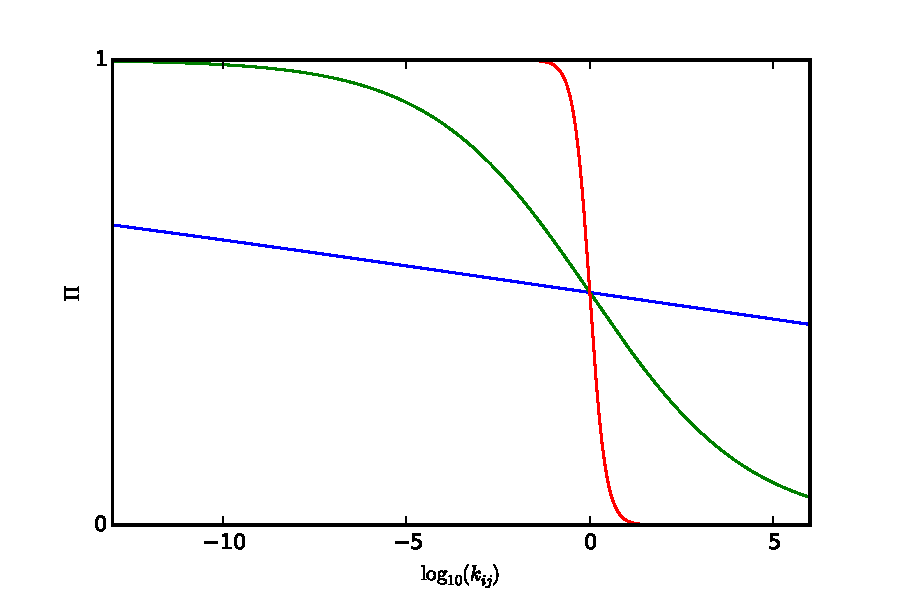
\includegraphics[width=0.7\textwidth]{./Plots/CaptureEfficiency.pdf}
 \caption[$\Pi$]{ Formas para $\Pi$ en escala logar\'itmica para distintos valores de $\phi$ , ({\hwplotB}) = 0.02 , ({\hwplotG}) = 0.2 y ({\hwplotR}) = 2 . Donde se observa que si $\phi_1 > \phi_2$ entonces $\Pi_{\phi_1}(k_{ij}) >\Pi_{\phi_2}(k_{ij})$ para $k_{ij} < 1$ y lo contrario en caso $k_{ij}>1$ }
 \label{fig:efficiency} 
\end{center}
\end{figure}

$d$ es el radio de detecci\'on m\'aximo a la cual un depredador de un tama\~no percibe a la presa, la relaci\'on con el tama\~no corporal se desprende del siguiente argumento:\\ Sea $\eta$ la agudeza visual del depredador $j$ y $\theta$ el \'angulo de resoluci\'on:
\begin{equation}\label{eq:d}
\begin{aligned}
\tan{\theta/2} &= \frac{L_{j}}{d} \\
\theta &= \frac{1}{\eta} \\
\eta & = c_a L_i^{b_a} \\
M &= c_{lm}L^{b_{lm}} 
\end{aligned}
\end{equation}
\subsubsection*{Donde:}
$L_i , L_j$ son las longitudes corporales del recurso $i$ y depredador $j$ respectivamente. \\La \'ultima relaci\'on expresa la alometr\'ia existente entre la longitud y la masa de una espacie, $b_{lm} \approx 3 $ y $c_{lm}$ es una constante que depende de la forma y densidad de la especie \citep{peters1986ecological,mcgill2006allometric}. \\
$b_a \approx 1 $ y $c_a$ varia dependiendo del grupo taxon\'omico y el ambiente \citep{kiltie2000scaling} .\\
\cite{pawar2012dimensionality} derivan $d$ de la siguiente relaci\'on:
\[ d = d_0(m_im_j)^{p_d} \]
La cual es una aproximaci\'on plausible derivada de \eqref{eq:d} y es la que nostros usamos. $d_0$ y $p_d$ son constantes que son influenciadas por la dimensi\'on del espacio de b\'usqueda $D$. \\
Realizando algunas simplificaciones en \eqref{eq:alfa} se llega a obtener la siguiente forma para la respectiva tasa de ataque $\alpha$ \citep{pawar2012dimensionality}.

\begin{equation}\label{eq:p4}
\begin{aligned}
&m_\C \alpha_1= \alpha_{0,1}m_\C^{p_v+2p_d(D_R-1)}f_1(k_{\RC})\\
&m_\PP \alpha_2= \alpha_{0,2}m_\PP^{p_v+2p_d(D_R-1)}f_2(k_{\RP})\\
&m_\PP \alpha_3= \alpha_{0,3} m_\PP^{p_v+2p_d(D_C-1)}f_3(k_{\CP})\\
\end{aligned}
\end{equation}
\subsubsection*{Donde:}
$p_v$ y $p_d$ son exponentes que controlan como escala la velocidad de un individuo  y la distancia de reacci\'on con el tama\~no corporal, respectivamente. El valor de $p_d$ var\'ia ligeramente con la dimensi\'on en la cual se desarrolla la interacci\'on \citep{pawar2012dimensionality}.\\
La funci\'on $f$ incorpora tanto los cambios sobre $S_A$ como $\aleph$ respecto a $k$ y a su vez es dependiente de la estrategia de forrajeo($Fm$) del depredador donde tres casos son considerados\citep{pawar2012dimensionality}.
\begin{itemize}
\item Captura activa ($Ac$).
\item Pastoreo ($Gr$).
\item Captura pasiva-\textit{Sit and wait}.($Sw$) 
\end{itemize}

\begin{equation}\label{eq:fkr}
f(k_{ij}) = 
\begin{cases}
\sqrt{1+k_{ij}^{2p_v}}k_{ij}^{(D_j-1)p_d} \Pi(k_{ij}) & Fm = Ac\\
k_{ij}^{p_v+(D_j-1)p_d}\Pi(k_{ij}) & Fm = Sw\\
k_{ij}^{(D_j-1)p_d}\Pi(k_{ij}) & Fm = Gr\\
\end{cases}
\end{equation}

Un an\'alisis del comportamiento de estas funciones se detalla en anexos \ref{subsec:funcf}.

\subsection{An\'alisis}
Todos los an\'alisis descritos a continuaci\'on se desarrollar\'an para el modelo descrito y con distintas combinaciones de dimensi\'on del habitat, estrategia de forrajeo,nivel de productividad ambiental basal y $\Pi$, las combinaciones usadas se especifican en Anexo \ref{subsec:params} .\\
Definiendo:
\begin{equation}
  k_\RC = \frac{ m_R}{m_C} \ \ \land k_\CP = \frac{m_C}{m_P}
\end{equation}
Como la \emph{raz\'on de masas presa-depredador},podemos expresar $m_R$ y $m_C$ en funci\'on a $m_P$ y la respectiva raz\'on de masas, esto sumado a la parametrizaci\'on empleada nos sirve para explorar los efectos que causan estos 3 par\'ametros sobre las propiedades del m\'odulo. Fijando las dem\'as constantes reducimos el espacio param\'etrico se reduce a tres ejes : $k_\RC,k_\CP, m_p$(note que $k_\RP = k_\RC k_\CP$). \\
A su vez se debe notar que aumentos en $m_P$ para un par de $k_\RC$ y $k_\CP$ fijos, aumentan la masa de las tres especies. 

\subsubsection{Criterios de Invasibilidad}\label{subsubsec:Inv}
Se delimitaron zonas dentro del espacio param\'etrico donde era posible la invasi\'on de una de las especies sobre un sistema receptor(debido a esto se les denomina \emph{criterios de invasibilidad}), para el sistema que estamos analizando los siguientes escenarios son posibles: 

\begin{itemize}
\item $R$ invade un sistema \emph{vac\'io}.
\item $C$ invade un sistema conformado solo por $R$.
\item $P$ invade un sistema conformado solo por $R$.
\item $P$ invade un sistema conformado por $R$ y $C$.
\item $C$ invade un sistema conformado por $R$ y $P$.
\end{itemize}
En los 3 primeros escenarios la variaci\'on de la longitud de la cadena tr\'ofica involucra al mecanismo de \textit{adici\'on} y en el \'ultimo escenario el mecanismo involucrado es el de \textit{inserci\'on}.\\

La derivaci\'on de estos criterios asume lo siguiente:
\begin{itemize}
\item \emph{El sistema receptor se ha encontrado aislado por suficiente tiempo como para alcanzar un estado asimpt\'otico y que dicho estado es un punto de equilibrio}.\\Esta suposici\'on es plausible ya que se espera que los eventos de inmigraci\'on de $C$ y $P$ no coincidan y que la separaci\'on entre ambos sea \emph{suficientemente} larga. M\'as a\'un en el modelo usado, en cualquier subsistema de dos especies(e.g $R-C$) la condici\'on inicial (e.g. $(R_0,C_0) \in R_2^+$) pertenece al dominio de atracci\'on del punto de equilibrio.(Dado que el sistema es \emph{volterra dissipative})
\item \emph{La invasi\'on se considera exitosa si es que existe un crecimiento por parte del invasor en los instantes posteriores a la invasi\'on}. *En el caso del sistema tridimensional esta condici\'on es necesaria para la invasi\'on.
\end{itemize}

Se calcularon 5 criterios de invasibilidad $\mathbf{I_{\R},I_{\C \to \R},I_{\PP \to \R},I_{\PP \to \C-\R},I_{\C \to \PP-\R}}$ y se asoci\'o a cada uno la zona del espacio param\'etrico explorado donde se cumplen, la zona asociada al criterio $I$ se denota por $\mathbf{Z(I)}$ .\\

Un ejemplo de la forma de calcular estos criterios se detalla a continuaci\'on, y los dem\'as se especifican en \ref{subsec:CI}

\myparagraph{P $\to$ C-R}

\begin{equation} \mathbf{IC_{\PP \to \C-\R}} := \dot{P} >0 \iff \epsilon_2\alpha_2\hat{R}_2 + \epsilon_3\alpha_3\hat{C}_2 > q_2 m_P \end{equation}

Donde:
\begin{equation}
\begin{aligned}
\hat{R}_2 &= \frac{q_1 m_C}{\epsilon_1 \alpha_1} \\
\hat{C}_2 &=  r(\frac{m_C}{\alpha_1}) \left[ 1 - \frac{q_1 m_C}{\epsilon_1 \alpha_1 K} \right] 
\end{aligned}
\end{equation}

\begin{equation}
\mathbf{Z(I_{\PP \to \C-\R})} := \{ v \in \mathbf{Z(I_{\C \to \R})} / \dot{P}(v) > 0 \}
\end{equation}


\subsubsection{Zonas de Coexistencia}
Se delimitaron zonas dentro del espacio param\'etrico donde el triple equilibrio $\mathbf{X} = (R^*,C^*,P^*)$ fuese positivo, $\mathbf{X}$ tiene la propiedad de que $N(\mathbf{X}) = 0$ para $N$ descrito en \eqref{eq:Gsystem}. El conjunto de los puntos de equilibrio es denotado por $E$.
\begin{equation}\label{eq:Equilibrio}
E:= \{ (R,C,P) \in \mathbf{R}^3_+ / N((R,C,P)) = 0 \}
\end{equation}

En nuestro caso las expresiones para el equilibrio son(el c\'alculo se detalla en \ref{subsec:equil}):
\begin{flalign}
R^* &= \frac{K(\epsilon_3 ( \alpha_2 q_1 + \alpha_3 r) - \alpha_1 q_2)}{A}& \\
C^* &= \frac{K\alpha_1 \alpha_2 \epsilon_1 q_2 - K \alpha_2 \epsilon_2 ( \alpha_2 q_1 + \alpha_3 r) + \alpha_3 q_2 r} {\alpha_3 A} \\
P^* &= \frac{K \alpha_1 (\alpha_2 \epsilon_2 q_1 + \alpha_3 \epsilon_1 \epsilon_3 r) - (K \alpha_1^2 \epsilon_1 q_2 + \alpha_3 \epsilon_3  q_1 r)}{\alpha_3 A }
\end{flalign}
Donde:
\begin{equation}
A = K \alpha_1 \alpha_2 (\epsilon_1 \epsilon_3 - \epsilon_2 ) + \alpha_3 \epsilon_3 r
\end{equation}
Manipulando algebraicamente $C^*$ y $P^*$ se deriva que la condici\'on para que $(R^*,C^*,P^*)$ pertenzca a $R^3_+$ es que se cumplan $I_{\C \to \PP-\R}$ y $I_{\PP \to \C-\R}$ en el caso que $A > 0$ y que no se cumplan ambos en caso que $A < 0$. Si $A = 0$ el sistema no posee equilibrio no trivial. \\
Dado lo descrito anteriormente en el caso que $A <0$ el equilibrio no puede formarse mediante ning\'un camino de ensamblaje con los supuestos hechos en \ref{subsubsec:Inv}.\\
 Denotamos :
\begin{equation}
  \begin{aligned}
    E_1 &= \{ n \in E / A > 0 \}  \\
    E_2 &= \{ n \in E / A < 0 \}
  \end{aligned}
\end{equation}

\myparagraph{Habilidad Competitiva}
Se puede derivar que una condici\'on necesaria para que el sistema tenga un equilibrio estable es la siguiente:
\begin{equation}
  \frac{q_2}{\varepsilon_2 \alpha_2 } > \frac{q_1}{\varepsilon_1 \alpha_1}
\end{equation}
Lo cual es equivalente a que $R^*_\PP < R^*_\C$ que denota una mayor habilidad competitiva por parte del consumidor intermedio seg\'un la \emph{regla R}\citep{Tilman1990}.

Con la parametrizaci\'on usada para una masa de depredador tope $m_P$ dada esta condici\'on se reduce a 
\begin{equation}
  \frac{q_{0,2}}{\varepsilon_2 \alpha_{0,2} f_2(k_{\RP})} > \frac{q_{0,1} k_{\CP}^{\beta-h}}{\varepsilon_{1} \alpha_{0,1} f_1(k_{\RC})}
\end{equation}

Donde $ h = p_v + 2(D_R -1) p_d$.

\subsubsection{Estabilidad Din\'amica}
Se determin\'o la influencia sobre la estabilidad local del punto de equilibrio dentro de la zona de coexistencia, el procedimiento se detalla en \ref{subsec:stab}.


\subsubsection{Longitud de cadena tr\'ofica}

Dentro de la zona de coexistencia, calculamos el valor de la m\'axima posici\'on tr\'ofica $MTP$ para el punto de equilibrio, esto es:
\begin{equation}
  MTP = \frac{ 2 \varepsilon_2 \alpha_2 R^* + 3 \varepsilon_3 \alpha_3 C^*}{ \varepsilon_2 \alpha_2 R^* + \varepsilon_3 \alpha_3 C^*} = 2 + \frac{\varepsilon_3 \alpha_3 C^*}{q_2}
\end{equation}

\subsection{An\'alisis da datos}

En base a la red tr\'ofica de Benguela \citep{yodzis1998:localTD} y los datos de masas coporarles publicados en \citet{brose2006:bodysizecr}. Extraemos de la red todos los triples de especies que conformen un m\'odulo IGP y para una gradiente de valores de $\kappa_0$ calculamos la proporci\'on de m\'odulos cumpliendo alguno de los criterios de invasibilidad o coexistencia respectivamente. 

\begin{figure}[!htbp]
  \centering
  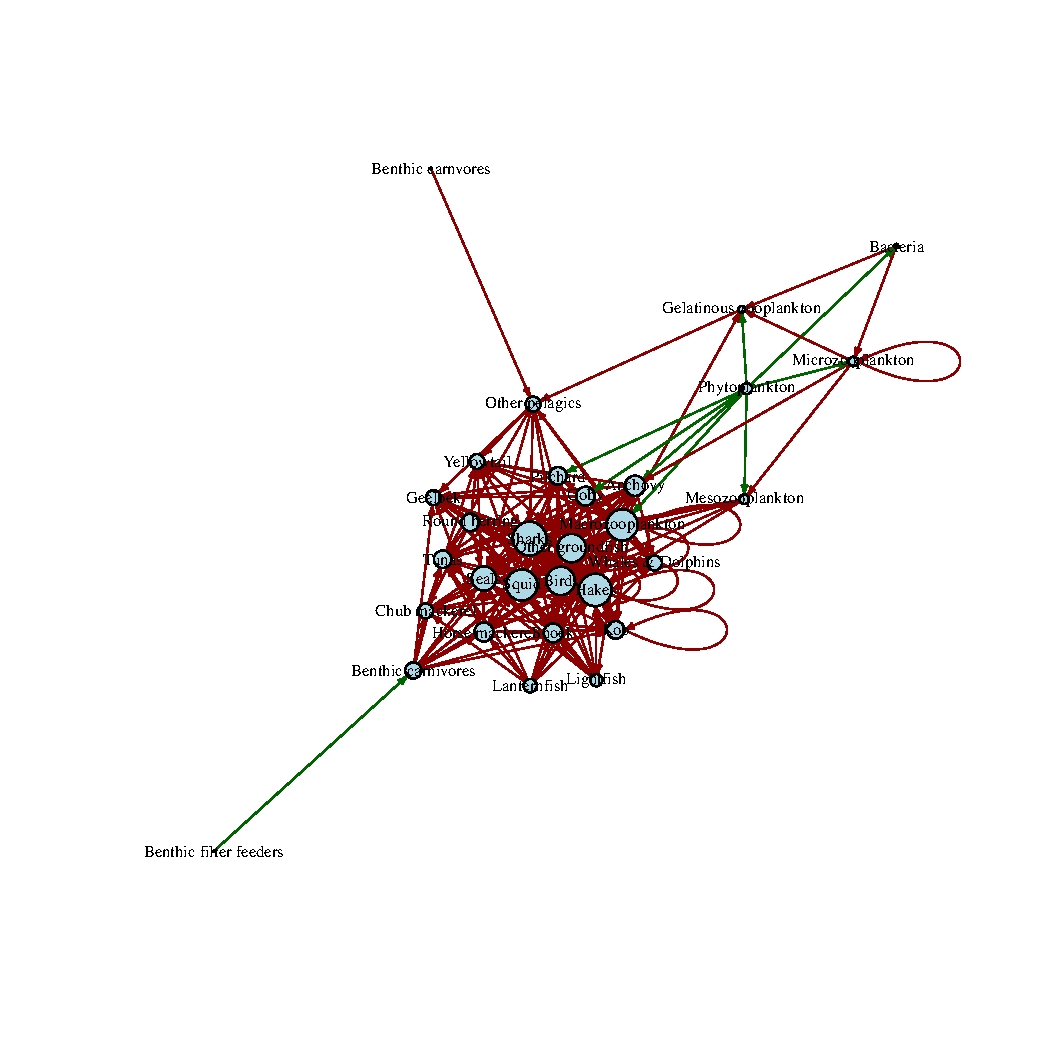
\includegraphics[width = 0.99\textwidth]{./Plots/Benguela.pdf}
  \caption[Benguela]{Red tr\'ofica de Benguela \citep{yodzis1998:localTD}}
  \label{fig:Benguela}
\end{figure}





\section{RESULTADOS}

\subsection{Invasibilidad}

Para una zona $Z$ en particular definimos la \emph{zona relativa} al tipo de comunidad $n$ como $Z_n = Z \cap C_n$. \\
A continuaci\'on se describen resultados para la combinaci\'on de estrategias de forrajeo \emph{Grazing-Grazing-Active}. Dado que en los otros dos casos se obtiene una respuesta cualitativa similar estos no ser\'an detallados.

\subsubsection{$ P \to R-C$}

En todos los casos explorados $Z(IC_4)$ tiende a crecer con respecto a aumentos en la masa del depredador $m_P$, y adem\'as forman una secuencia encajante. Dicho crecimiento es en cierta manera similar al que experimenta una zona para una valor de $m_P$ en particular, respecto a aumentos en la productividad basal $k_0$. Sin embargo el crecimiento no es uniforme, las zonas relativas si bien tienden a crecer lo hacen de manera desigual dependiendo adem\'as del valor del par\'ametro $\phi$.\\

El valor de $\phi$ controla en cierta manera la forma de $Z(IC_4)$, observandose por lo general una relaci\'on inversa del valor de $phi$ y el \'area total de $Z(IC_4)$ irrespectivamente de la masa. Sin embargo afecta de manera desigual los distintos tipos de Comunidades.\\ Por ejemplo, en el caso de comunidades con distribuci\'on de masa $C_1$ el par\'ametro es pr\'acticamente irrelavante sobre la zona relativa $Z(IC_4)_1$, y por el contrario para comunidades $C_5$ el cambio es dram\'atico, dado que entre $\phi  = 0.02 - 2$, $Z(IC_4)_5$ pasa de ser no vac\'ia y cubrir en su totalidad(en el caso 3D) a $C_5$ (i.e $Z(IC_4)_5 = C_5$) para todas las masas $m_P$ exploradas, a ser vac\'io para todo $m_P$ en el segundo caso.\\
La dimensi\'on del espacio de b\'usqueda afecta el \'area total y las \'areas relativas de $Z(IC_4)$.\\
En el primer caso observamos que generalmente es mayor en espacios tridimensionales(3D) y esta diferencia se acent\'ua conforme la masa $m_P$ aumenta.\\
En el segundo caso tenemos un patr\'on muy similar pero en este caso para $m_P$ bajos se pueden observar comunidades donde el \'area de la zona relativa es mayor en ambientes bidimensionales, como por ejemplo $Z(IC_3)$ para $m_P = 10^{-10}$. \\
Adem\'as tenemos que la distribuci\'on del \'area de las zonas \emph{relativas} es diferente en espacios 3D y 2D.\\
Algo que resaltar es que el borde inferior(en escala logar\'itmica) tiende a ser \emph{paralelo} a $\log_{10}(K_{CP}) = -log_{10}(K_{RC})$ en el caso 3D y no en el caso 2D.


\begin{figure}
  \centering
  \includegraphics[width = 0.9\textwidth]{./Plots/ZIC4b2e0.pdf}
  \caption[Env $Z(IC4)$]{\emph{Envolturas de Invasibilidad} para el caso de el depredador tope $P$ como invasor frente a una comunidad receptora formada por $R-C$. La fila superior es para espacios de b\'usqueda bidimensionales y la inferior tridimensionales, las columnas de izquierda a derecha aumentan el nivel de productividad basal $k_0$, siendo $0.01,0.1,1$ y $3,30,300$ en la primera y segunda fila respectivamente.Las diferentes lineas implican distintas masas de depredador $m_P$ :({\hwplotR}) $10^5 kg$,  ({\hwplotY}) $1kg$, ({\hwplotG}) $10^{-5}kg$ y ({\hwplotB}) para $10^{-10}kg$. ({\hwplotK}) separa las zonas donde $K_{RC},K_{CP},k_{RP}$ son mayores o menores que 1 respectivamente.}
  \label{fig:Z(IC4)}
\end{figure}

\subsubsection{$C \to R-C$}
De forma similar al caso anterior tenemos que el \'area total de $Z(IC_5)$ esta relacionada positivamente con el valor de $m_P$, sin embargo a diferencia del caso anterior las zonas para distintos $m_P$ si bien tienen intersecci\'on no vac\'ia ,no forman una secuencia encajante. Es decir a parte de crecimiento tenemos un desplazamiento conforme aumenta $m_P$. Igual que en el caso anterior este patr\'on se asemeja al observado para un $m_P$ en particular respecto a la variaci\'on de $k_0$. \\
En este caso es bastante notorio la no uniformidad en el \'area de las zonas relativas.\\

El par\'ametro $\phi$ juega un papel importante en la topolog\'ia de $Z(IC_5)$, para valores peque\~nos el conjunto es conexo, sin embargo para $\phi = 2$ el conjunto tiene 2 componentes, caracterizadas por la distribuci\'on de sus \'areas relativas. La distancia entre estas componenes aumenta con $m_P$ y $k_0$ , para $m_P$($k_0$) elevados podemos distinguirlas por el hecho que una de ellas $\vartheta_C^1$intersecta principalmente las zonas $C_4,C_5,C_6$ y la otra $\vartheta_C^2$ las zonas $C_1,C_2$, siendo la primera la que presenta mayor \'area. \\
Para $\phi = 0.2 ,0.02$  tenemos que $Z(IC_5)$ intersecta principalmente a las zonas $C_2,C_3,C_4$ y posee una \emph{cola} que es paralela(en escala logar\'itmica) a $\log_{10}(K_{CP}) = -log_{10}(K_{RC})$ y que dependiendo del valor de $m_P$($k_0$) esta contenido en las zonas $C_1,C_2,C_6$ o $C_3,C_4,C_5$, es decir $k_{RP} > 1$ o $k_{RP}<1$. \\

La dimensi\'on del espacio de b\'usqueda igual que en el caso anterior afecta el \'area total de $Z(IC_5)$ la cual es mayor en ambientes tridimensionales. Sin embaro la distribuci\'on de las zonas \emph{relativas} es similar en los dos casos. \\
Para $\phi = 2$ se observa que el \'area de $\vartheta_C^2$ es por lo general mayor en ambientes bidimensionales y lo contrario ocurre con el otro componente.

\begin{figure}
  \centering
  \includegraphics[width = 0.9\textwidth]{./Plots/ZIC5b2e0.pdf}
  \caption[Env $Z(IC5)$]{\emph{Envolturas de Invasibilidad} para el caso de el depredador intermedio $C$ como invasor frente a una comunidad receptora formada por $R-P$. Las dem\'as especificaciones se comparten con la figura ~\ref{fig:Z(IC4)}.}
\end{figure}























\section{DISCUSION}


Nuestros resultados muestran que dependiendo de la combinanci\'on de masas presente en el m\'odulo IGP el curso del ensamblaje del m\'odulo puede tomar distintos caminos, en particular se observa que ciertas combinaciones restringen la \emph{adici\'on} de depredadores(tope o intermedio) o la \emph{inserci\'on} del depredador intermedio restringiendo de esta manera posibles cambios en la FCL observada en la comunidad. Estas observaciones complementan el trabajo realizado por \citet{holt2002food} en el cual sugiri\'o el hecho que procesos espaciales como \emph{colonizaci\'on} o \emph{extinci\'on} ser\'ian limitantes de FCL, para ser m\'as precisos estos procesos estar\'ian modulando la estructura de la \emph{red tr\'ofica} presente en la comunidad y a su vez la estructura en un instante determinado limita colonizaciones o extinciones futuras\citep{pawar2009community,holt2002}.  Los resultados obtenidos en este trabajo sugieren que esta \emph{feed-back} entre la estructura de la red y el procesos de ensamblaje estar\'ia a su vez influenciado por la distribuci\'on de masas presentes tanto en la comunidad receptora como en el pool de colonizadores.\\

Dada la influencia que tiene la masa corporal de las especies sobre la tasa de metabolismo(citar), y su subsecuente influencia sobre para\'ametros tanto \emph{intra}($r,K,q_0$)  e \emph{inter-poblacionales} ($\alpha_i$) es plausible pensar que la distribuci\'on de masas tendr\'ia un efecto sobre los mecanismos de invasibilidad y las zonas de coexistencia del m\'odulo IGP , irrespectivamente de las particularidades del modelo usado(e.g respuesta funcional Tipo I). \\

La similaridad en la variaci\'on en el \'area total de todas las zonas con respecto a aumentos en $m_P$ y $k_0$ estar\'ia indicando que el mayor efecto que tiene $m_P$ sobre la invasibilidad es el hecho de aumentar la capacidad de carga de $R$ y esto se debe al hecho de que si bien $m_P$ afecta el valor de diversos par\'ametros del modelo(e.g tasas de mortalidad $q$) las constantes que acompa\~nan a dichos par\'ametros son relativamente peque\~nas comparadas con $k_0$.\\
En nuestros resultados $m_P$ cumple el papel de reescalar los valores posibles de masas presentes en la comunidad, es decir $m_P$ mayores implican un mayor valor de $m_R$ y $m_C$ para una determinada combinaci\'on de $k_{\RC}$ y $k_{\CP}$. Para un $m_P$ en particular los limites de las zonas de invasibilidad estan relacionados con limitaciones energ\'eticas, dado que al momento de invadir la principal prioridad del invasor es alcanzar la cantidad de energ\'ia necesaria para subsistir en el ambiente, dicha limitaci\'on se observa en el hecho de que combinaciones con valores muy peque\~nos de $k_{\RC}$ y $k_{\CP}$ son excluidos en todos los casos explorados, y otra prueba de esto es el hecho que al aumentar la energ\'ia total disponible en el sistema o la tasa de adquisici\'on de energ\'ia, mediante aumentos en $k_0$ o $m_p$ , mayor proporci\'on de combinaciones en la comunidad $C_1$ son incluidas en las zonas de invasibilidad y coexistencia.\\


El par\'ametro $\phi$ va afecta el modo en el que los \emph{size ratios} $k_{ij}$ afectan a la tasa de consumci\'on por parte de los depredadores,como se observa en \ref{fig:efficiency} para valores de $k_{ij}$ mayores a 1 valores de $\phi$ elevados afectan negativamente la eficiencia de captura($\Pi$) y lo contrario se observa para $k_{ij} <1$. Para valores bajos(0.2 y 0.02 en nuestro caso) el efecto positivo que causa el que la presa sea mas grande(debido a un mayor movimiento (en caso de \emph{active} y \emph{sit and wait} strategies) y a un incremento en la energ\'ia disponible) domina al efecto negativo que causa $k_{ij}$ sobre la eficiencia de captura. Sin embargo para $\phi = 2$ tenemos que el efecto negativo es el que domina en valores elevados de $k_{ij}$. Esto se aprecia tanto por el hecho de que valores elevados de \emph{size ratios} son excluidos en el caso de $Z(I_{\C \to \R}),Z(I_{\PP \to \R}),Z(I_{\PP \to \C-\R})$ y adheridos en el caso de $Z(I_{\C \to \PP -\R})$ donde un valor elevado de $k_{\CP}$ implica una menor eficiencia en su captura por parte del deprador tope lo cual posibilita su invasi\'on al sistema. A su ves el valor de este par\'ametro controla la conexidad de las zonas de coexistencia, inserci\'on e invasibilidad mutua lo cual implica la posibilidad de tener una bimodalidad en los \emph{size ratios} encontrados en una comunidad compuesta por m\'as de un m\'odulo IGP asociadas incluso con una misma masa de depredador tope $m_P$.\\

Adem\'as observamos que cualitativamente las influencias de $m_p$ ,$k_0$ y $\phi$ sobre las zonas de invasibilidad y coexistencia son similares para las tres combinaciones de estrategia de forrajeo usadas, y como se observo en un an\'alisis previo\citep{pawar2012dimensionality} , la diferencia entre las zonas para las distintas combinaciones es menor comparada con la diferencia causada por distinta dimensi\'on de b\'usqueda. Esta \'ultima es causada por los cambios que se producen sobre la regi\'on de detecci\'on del depredador y la asociaci\'on de espacios de busqueda de dimensi\'on diferente con ambientes con diferentes tasas de productividad basal. \\


La zona de \emph{coexistencia inestable}(pero que la cual en principio puede formarse mediante una secuencia de invasiones), es extremadamente peque\~na lo cual estar\'ia indicando que para una parametrizaci\'on biol\'ogicamente realista si una combinaci\'on de masas presenta un equilibrio este con gan probalidad ser\'ia estable, es de resaltar que las comunidades asociadas con esta zona de coexistencia son las $C_3,C_4$ donde el depredador tope es mas peque\~no que sus presas cosa que concuerda con resultados previamente reportados(citar Martinez,Yodzis) que sugieren que depredadores peque\~nos al tener una mayor tasa de metabolismo por unidad de masa tienden a generar inestabilidades.El parametro $\phi$ tiene una influencia positiva sobre la estabilidad y al valor de 2 tenemos que toda la zona de coexistencia es estable, debido a como se dijo en el p\'arrafo anterior su influencia sobre la optimalidad de los size ratios, la cual restringe la inclusi\'on de valor extremos.


Es de resaltar que la zona de mutua invasibilidad es relativamente peque\~na lo que nos dice que existe una gran restricci\'on sobre las combinaciones de masas que har\'ian posible al modulo tener esta cualidad de ``\emph{bi-ensamblaje}'', nuestros resultados complementan resultados anteriores que relacionaron la distribuci\'on de masas con la estabilidad din\'amica del sistema(citar martinez) y a su ves muestran como un factor end\'ogeno puede modular la expresi\'on de los mecanimos de variaci\'on de la posici\'on tr\'ofica presente y que en cierta manera modular\'ia los efectos que producen factore ex\'ogenos que son los comunmente explorados(e.g tama\~no del ecosistema), y como se observa esta modulaci\'on es debido a cambios a nivel individual(metabolismo, movimiento) que escalan a propiedades interespec\'ificas(invasibilidad), esta forma de modular la longitud implica que para ambientes con caracter\'isticas f\'isicas similares pero con distinta distribuci\'on de masas en el pool regional (i.e pool de potenciales colonizadores) podemos esperar diferencias tanto en la historia de ensamblaje de la comunidad como en la m\'axima posici\'on tr\'ofica.



\section{Conclusiones}

La distribuci\'on de masas presente en una comunidad modula la longitud de la cadena tr\'ofica, debido a su influencia sobre los mecanismos de ensamblaje y coexistencia de las especies, las relaciones existentes se basan en la forma en que las masas afectan la tasa de p\'erdida y adquisici\'on de energ\'ia de las especies involucradas.\\
La forma de las relaciones ($\mu_i$) es independiente de la productividad del ambiente, la dimensi\'on del espacio de b\'usqueda y la combinaci\'on de estrategias de forrajeo; sin embargo estas afectan el valor de $\zeta_i$ y $\gamma_i$. La acci\'on de los dos \'ultimos a su vez puede cambiar la forma de la respuesta de $\zeta_i$ y $\gamma_i$ respecto a cambios en $(k_\RC,k_\CP)$ y se observa un mayor efecto por parte de la dimensi\'on del espacio de b\'usqueda.\\
La influencia de la distribuci\'on de masas sobre el curso del ensamblaje de la comunidad (y la red tr\'ofica asociada) presenta un \'area de investigaci\'on muy prometedora y que a\'un no recibe la adecuada atenci\'on, esto a su vez podr\'ia acoplarse a la influencia que dicha distribuci\'on presenta sobre el funcionamiento del ecosistema a lo largo del proceso de ensamblaje. Resultados asociados a estos estudios ser\'ian de gran importancia no s\'olo desde el punto de vista te\'orico sino aplicado.






\bibliographystyle{abbrvnat}
\bibliography{BibliografiaTesis}

\newpage
\section{ANEXOS}
\subsection{Influencia de $k_{ij}$ sobre $f$}

Sin importar la estrategia de forrajeo tenemos que :
\begin{enumerate}[label=(\alph*)]
\item \begin{equation}
  \lim_{k_{ij} \to  0 }f(k_{ij}) = \lim_{k_{ij} \to 0 }\frac{g(k_{ij}) a}{1+k_{ij}^\phi} = 0 
\end{equation}
ya que $ g(k_{ij}) \to (k_{ij} \to 0)$ y $\frac{a}{1+k_{ij}^\phi} < a$  para todo $k_{ij}$
\item 
\begin{equation}
\lim_{k_{ij} \to  0 }f(k_{ij}) - ag(k_{ij}) = 0
\end{equation}
y por lo tanto $f \approx a g(k_{ij})$ para $k_{ij}$ suficientemente peque\~no , donde $g(k_{ij}) = f(k_{ij})\Pi(k_{ij})$.
\item $f_{3D} > f_{2D} \iff k_{ij} > 1$ donde $f_{nD}$ representa al valor de $f$ para espacios de b\'usqueda \emph{n-dimensionales}
\end{enumerate}

A continuaci\'on se analizan propiedades de $f$ que a nivel \emph{cuantitativo} difieren entre las distintas estrategias de forrajeo

\subsubsection{Grazing}

\begin{prop}
  $f$ tiene un punto m\'aximo en $\mathbb{R}^+$ si y solo s\'i $\phi > (D_i - 1)p_d$ 
\end{prop}

\begin{proof}
\mbox{}\\
Sea $ h = (D_i-1)p_d$\\
Dado que $f$ es diferenciable y:
  \begin{equation}
    \begin{aligned}
      f'(k_{ij}) &= a \frac{h k_{ij}^{h-1} (1 + k_{ij}^\phi) -\phi k_{ij}^{\phi-1+h}}{(1+k_{ij}^{\phi})^2} \\
            &= a \frac{(h-\phi)k_{ij}^{h-1 + \phi}  + h k_{ij}^{h-1} }{(1+k_{ij}^{\phi})^2}\\
            &= a \frac{(h-\phi)k_{ij}^\phi + h }{(1+k_{ij}^{\phi})^2}\\
     \end{aligned}
  \end{equation}
Luego tenemos que $f'$ posee un \emph{cero} en $\mathbb{R}^+$ si y solo s\'i $ h< \phi$ y en caso afirmativo tenemos que $k^*$ tal que $f(k^*) = 0$ es $(\frac{h}{\phi-h})^{\frac{1}{\phi}}$ adem\'as:
\begin{equation}
  f'(x) :
  \begin{cases}
    < 0 &; k_{ij}  > k^* \\
    > 0 &; k_{ji} < k^*
  \end{cases}
\end{equation}

Lo que indica que $k^*$ es un punto m\'aximo.
\end{proof}

De la proposici\'on anterior tambi\'en vemos la dependencia de $k^*$ en $\phi$, teniendo $h$ fijo en nuestro caso se observa que si $\phi$ esta suficientemente cercano a $h$ , $k^*$ es extremadamente grande, sin embargo se observa un decaim\'iento muy r\'apido y para valores de $\phi \geq 2h$  , $k^*$ se encuentra pr\'oximo a 1(y en realidad converge a 1 para $\phi \to \infty$) , v\'ease figura \ref{fig:kmaxGrazing}. \\

\begin{figure}
\begin{center}
 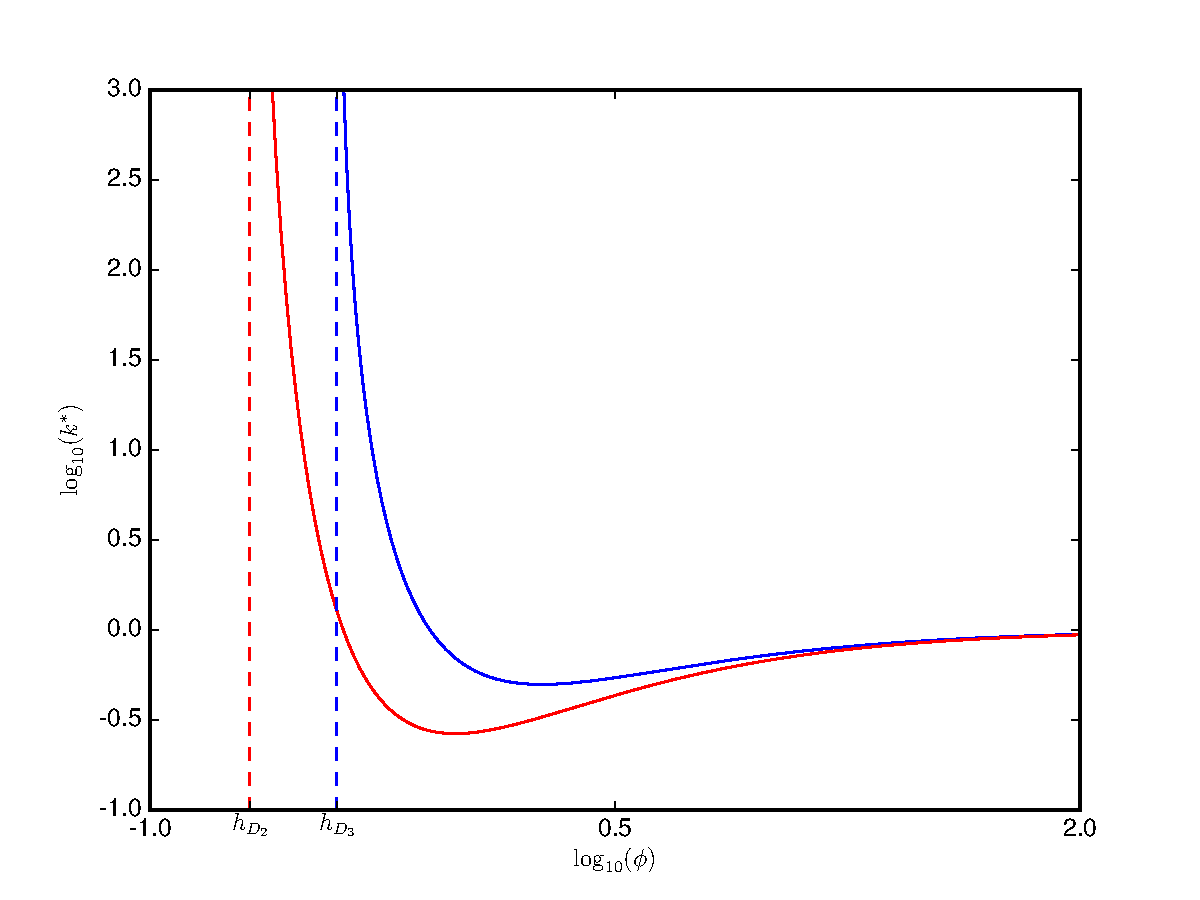
\includegraphics[width=0.9\textwidth]{./Plots/kmaxGrazing.pdf}
 \caption[$k^*, Grazing$]{$k^*$ en funci\'on a $\phi$ donde se observa la divergencia para valores cercanos a $h$ y la convergencia a 1 para valores elevados de $\phi$, ({\hwplotB}) es para el caso de ambientes de b\'usqueda $3D$ y ({\hwplotR}) $2D$, $h_{3D}$ y $h_{2D}$ denotan los l\'imites inferiores para $\phi$ que permiten la existencia de $k^*$}
 \label{fig:kmaxGrazing} 
\end{center}
\end{figure}



En el caso que $\phi < h$ tenemos que $f$ es mon\'otona creciente. Ambos casos se grafican en la figura \ref{fig:f1Grazing}.

\begin{figure}
\begin{center}
 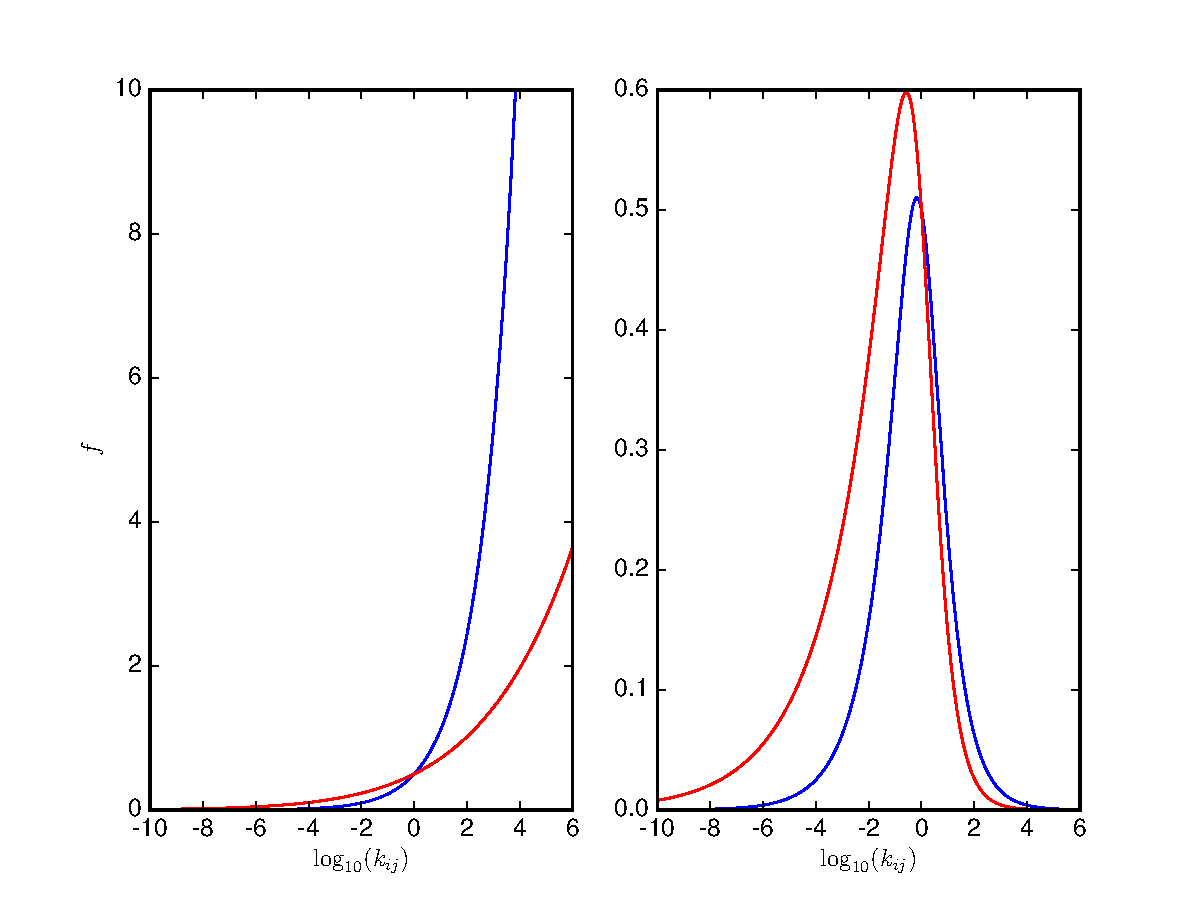
\includegraphics[width=0.9\textwidth]{./Plots/f1Grazing.pdf}
 \caption[$f_1, Grazing$]{$f$ en funci\'on a $k_{ij}$, con $a =1$, en el panel de la izquierda tenemos $b = 0.1$ y en el de la derecha $b=1.$ , ({\hwplotB}) es para el caso de ambientes de b\'usqueda $3D$ y ({\hwplotR}) $2D$}
 \label{fig:f1Grazing} 
\end{center}
\end{figure}


\subsubsection{Sit}

Se tiene cualitativamente las m\'ismas caracter\'isticas que en el caso anterior, con la diferencia que en este caso $ h:= p_v + 2(D_i -1) p_d$, y por ende para $\phi \in ]2(D_i - 1) p_d , p_V + 2(D_i -1)p_d[$ tendr\'iamos un comportamiento mon\'ontono para $f_{sit}$ y la existencia de un m\'aximo para $f_{grazing}$.\\

La figura \ref{fig:f1Sit} muestra las semejanzas con el caso anterior, salvo la diferencia que en este caso $k^*>1$ para el caso $3D$ y adem\'as alcanza un valor m\'as alto que el caso $2D$.\\
En general tenemos que $ k^*_{Sit} > k^*_{grazing}$ .

\begin{figure}
\begin{center}
 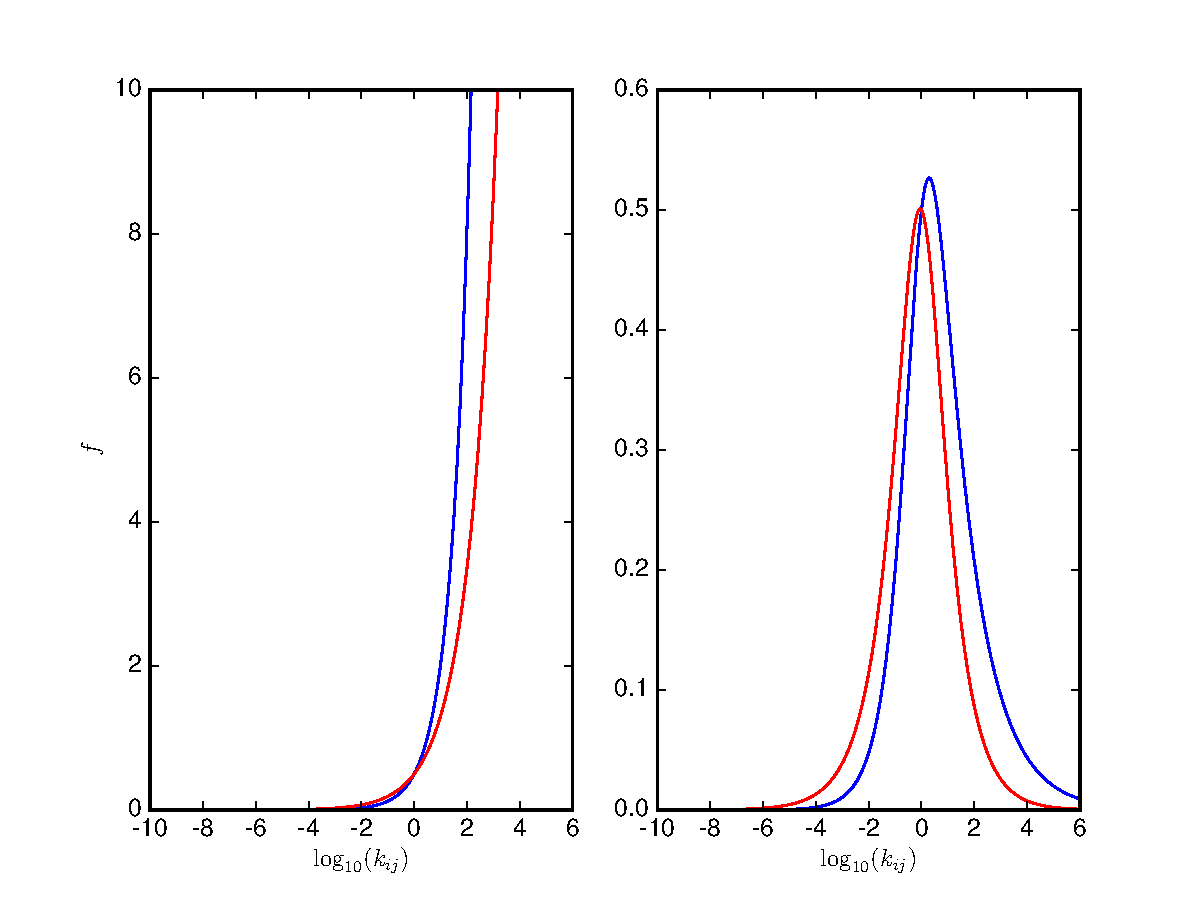
\includegraphics[width=0.9\textwidth]{./Plots/f1Sit.pdf}
 \caption[$f_1, Sit$]{$f$ en funci\'on a $k_{ij}$, con $a =1$, para el caso de una estrategia de forrajeo \emph{Sit-and-Wait}, las dem\'as especificaciones se comparten con la figura \ref{fig:f1Grazing}}
 \label{fig:f1Sit} 
\end{center}
\end{figure}


\subsubsection{Captura activa}

En este caso tenemos un comportamiento similar al descrito previamente, esto es para $\phi > p_v + 2(D_i -1) p_d$ tenemos que $f$ decae exponencialmente a partir de un valor de $k_{ij}$ \emph{suficientemente grande}, y a su vez crece exponencialmente para valores \emph{suficientemente peque\~nos}, dado que $f \in C^1$ esto a su vez nos dice que debe existir un punto m\'aximo para $f$ sin embargo en este caso no tenemos una expresi\'on an\'alitica para $k^*$ salvo que cumple la siguiente relaci\'on:

\begin{equation}
  (k^*)^{\phi}((k^*)^{2p_v}(p_v+ h -\phi) + (h -\phi) + (k^*)^{2p_v - \phi}(p_v + h ) ) + h = 0
\end{equation}

Con $h$ igual que en el caso $grazing$.\\
De esta relaci\'on podemos obtener que :
\begin{equation}
  k^*_{Active} \in ] k^*_{Grazing} , k^*_{Sit} [
\end{equation}

A su vez para $\phi \leq 2(D_i - 1)p_d $ podemos esperar un crecimiento mon\'otono por parte de $f$. 

\begin{figure}
\begin{center}
 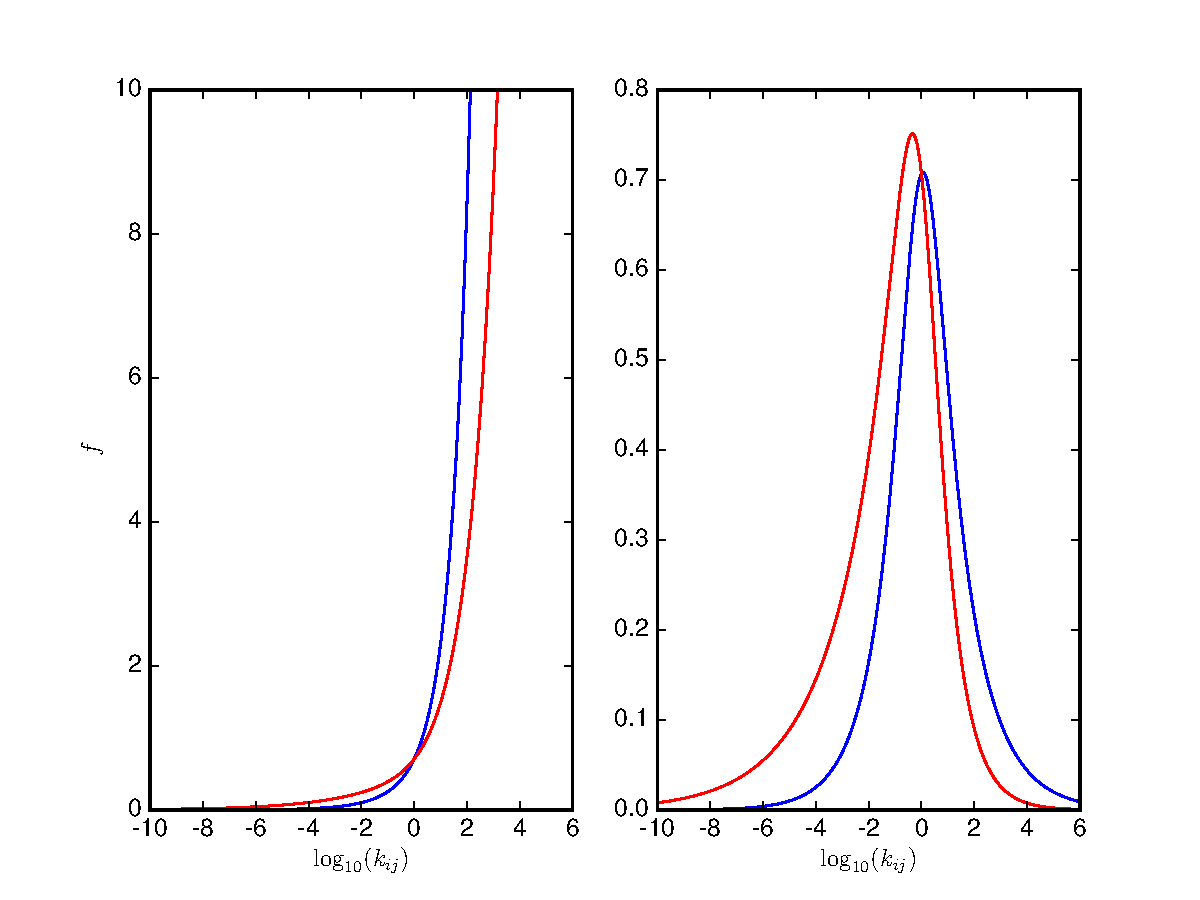
\includegraphics[width=0.9\textwidth]{./Plots/f1Active.pdf}
 \caption[$f_1, Active$]{$f$ en funci\'on a $k_{ij}$, con $a =1$, para el caso de una estrategia de forrajeo \emph{activa}, las dem\'as especificaciones se comparten con la figura \ref{fig:f1Grazing}}
 \label{fig:f1Active} 
\end{center}
\end{figure}




\subsection{Influencia de las masas sobre estados de equilibrio de las comunidades receptoras}

A continuaci\'ion usamos la notaci\'on empleada en resultados siempre que sea posible.
\subsubsection{R-C}
Tenemos que al equilibrio $R$ y $C$ estan determinados por el siguiente par de expresiones
\begin{equation}
  \begin{aligned}
    R_{eq} &= \frac{q_{0,1} m_C^{\beta-h}}{\varepsilon_1 \alpha_{0,1} f_1(k_\RC)}\\
    C_{eq} &= \frac{r_0 m_C^{\beta -h}}{\alpha_{0,2} k_\RC^{1 - \beta}f_1(k_\RC)}(1 - \frac{R_{eq}}{\kappa_0 (k_\RC m_C)^{1-\beta}})
  \end{aligned}
\end{equation}

Las condiciones de existencia de equilibrio positivo son equivalentes a las condiciones para la invasi\'on de $C$ y se detallan en Resultados.\\
Dentro del espacio param\'etrico que posibilita la coexistencia tenemos asu vez que el efecto que causa cambios en $m_C(k_\CP m_P)$ es dependiente de la dimensi\'on del espacio de b\'usqueda: para espacios $3D$ tiene un impacto negativo sobre $R_{eq}$ y lo contrario ocurre en el caso $2D$. Su influencia sobre $C_{eq}$ es mas dif\'icil de diferenciar , en el caso $2D$ tenemos que el impacto es positivo, sin embargo en $3D$ depende del valor de $m_C$ ya que:
\begin{equation}
  \frac{\partial C_{eq}}{\partial m_C}  = d_0 ( (b-h) + (1 + 2h - 3 \beta )\frac{\chi_1}{\chi_0} m_C^{2\beta -h -1}) 
\end{equation}
Entonces la regi\'on de crecimiento y decrecimiento respecto a $m_C$ esta determinada por:
\begin{equation}
  \begin{cases}
    Crecimiento &  m_C^{1 + h - 2\beta} < \frac{q_{0,1}(1+2h -3 \beta)}{\chi_0(h - \beta)}\\
    Decrecimiento &  m_C^{1 + h - 2\beta} > \frac{q_{0,1}(1+2h -3 \beta)}{\chi_0(h - \beta)}
  \end{cases}
\end{equation}

\begin{figure}
  \centering
  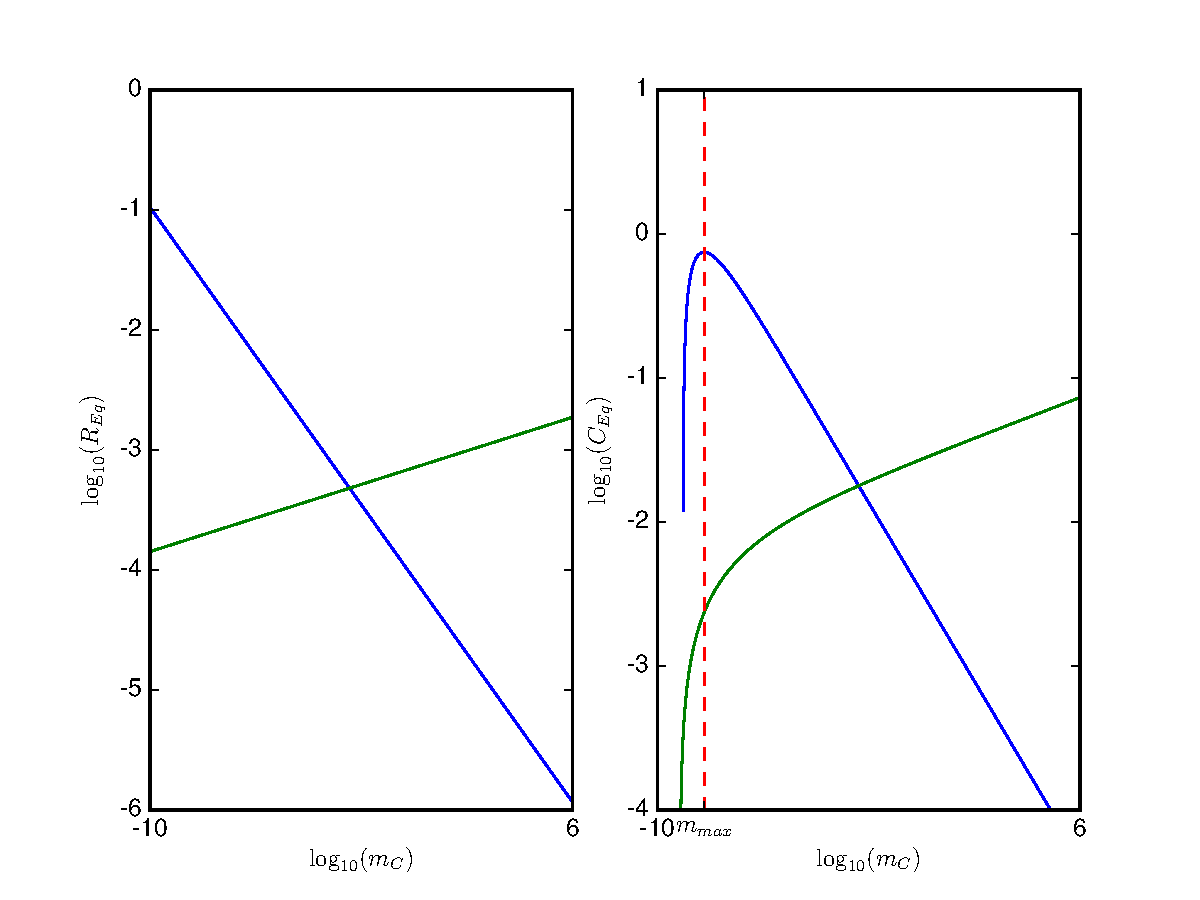
\includegraphics[width = 0.99\textwidth]{./Plots/RCeq.pdf}
  \caption[Equilibrio $R-C$vs$m_C$]{Equilibrios para el subsistema $R-C$ en funci\'on a $m_C$ para $k_\RC = 10^{-2}$, donde se observa las diferencias existentes entre espacios de b\'usqueda $2D$({\hwplotG}) y $3D$ ({\hwplotB}), en el panel de la derecha se representa a su vez el valor de $m_C$ para el cual $C_{eq}$ es m\'aximo.$b = 0.1$,$\kappa_0 = 0.1 , 30$  en espacios $2D$ y $3D$ respectivamente.}
  \label{fig:EqRCmC}
\end{figure}

La influencia de $k_\RC$(para un $m_C$ fijo)sobre los valores de equilibrio es an\'aloga a su influencia sobre la invasibilidad de $C$, dentro de la zona de coexistencia afecta negativamente a $R_{eq}$ en la zona de crecimiento de $f$ y positivamente en la zona de decrecimiento(si existiera), es decir se espera un valor m\'aximo de $R_{eq}$ para valores de $k_\RC$ cercanos a los l\'imites de coexistencia, la influencia sobre $C_{eq}$ al igual que en el caso anterior m\'as complicada teniendo:
\begin{equation}
  \frac{\partial C_{eq}}{\partial k_\RC}  = \frac{e_0 g'(k_\RC) }{g(k_\RC)^2} ( -1  + \frac{2e_1}{g(k_\RC)})
\end{equation}
Donde:
\begin{equation}
  \begin{aligned}
    e_0 &=  \frac{r_0 m_C^{\beta -h}}{\alpha_{0,2}} \\
    e_1 &=  \frac{q_{0,1} m_C^{2\beta-h-1}}{\varepsilon_1 \alpha_{0,1} \kappa_0}
  \end{aligned}
\end{equation}

Por tanto:
\begin{equation}
  \begin{cases}
    Crecimiento &  g'(k_\RC) ( \frac{2e_1}{g(k_\RC)} - 1) > 0 \\
    Decrecimiento &  g'(k_\RC) ( \frac{2e_1}{g(k_\RC)} - 1) < 0
    \end{cases}
\end{equation}

Dado que $g'(k_\RC)$ es positivo para $k_\RC$ peque\~nos y a su vez $g(k_\RC)$ disminuye , podemos esperar que para $k_\RC$ suficientemente peque\~nos $k_\RC$ afecte positivamente a $C_{eq}$ ,por otro lado dependiendo del valor de $\phi$ y la estrategia de forrajeo podemos tener un comportamiento cualitativo diferente para valores intermedios de $k_\RC$, en el caso m\'as simple $g'(k_\RC)$ siempre es positivo y por ende solo existir\'ia un punto de transici\'on entre zona de crecimiento y decrecimiento dado por la condici\'on $g(k_\RC) = 2e_1$ , sin embargo en el caso que $g(k_\RC)$ posea a su vez zonas de crecimiento y decrecimiento, observar\'iamos 3 transiciones $k_\RC^1 , k_\RC^2$ y$k_\RC^3$ , determinadas por $g(k_\RC^1) = 2e_1$ , $g'(k_\RC^2) =0$ y $g(k_\RC^3) = 2e_1$ , esto siempre que $k_\RC^1 < k_\RC ^2 < k_\RC^3$ ,es decir siempre que $g$ crezca los suficiente, en este caso observamos que $\kappa_0$ y $m_C$ favorecer\'ian la existencia de estos puntos debido a su influencia negativa sobre $e_1$.


\begin{figure}
  \centering
  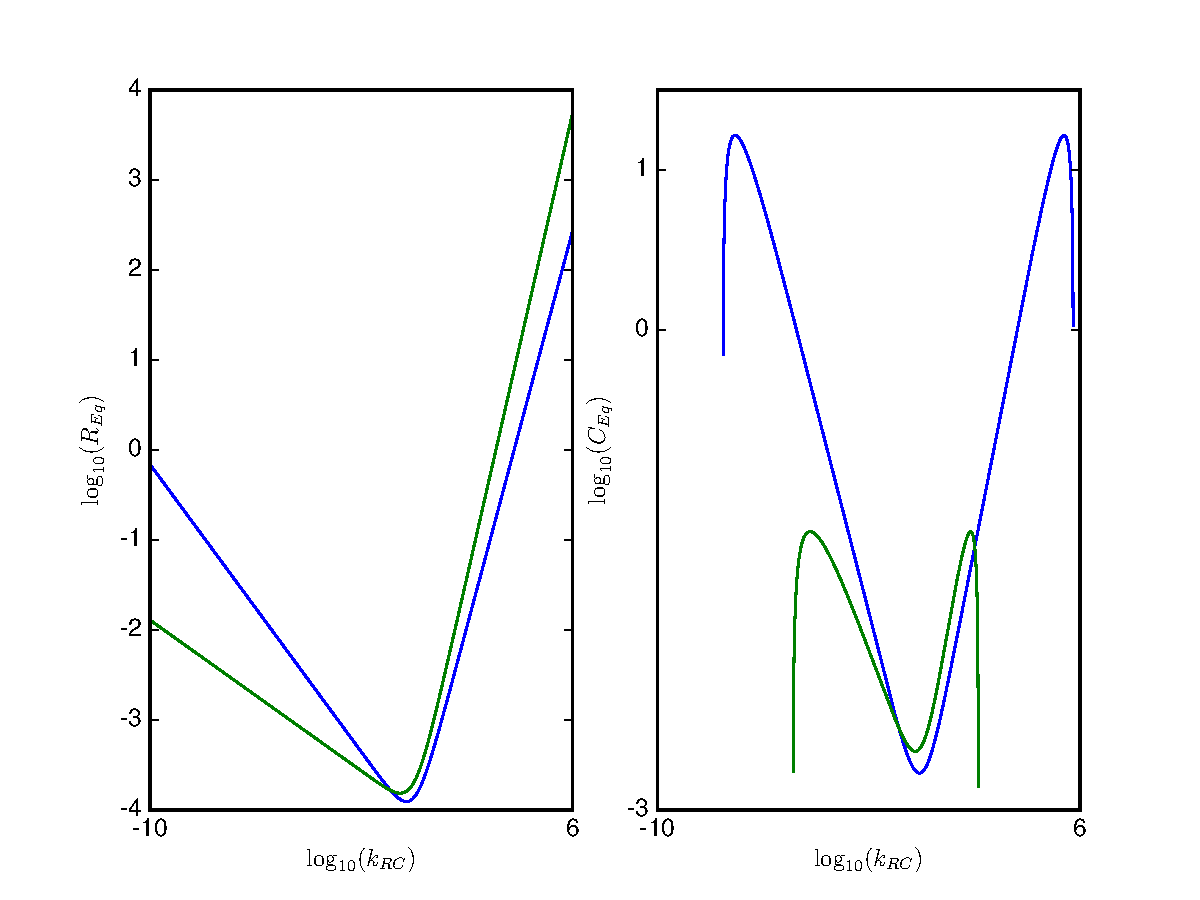
\includegraphics[width = 0.99\textwidth]{./Plots/RCeqKRC.pdf}
  \caption[Equilibrio $R-C$vs$k_\RC$]{Equilibrios para el subsistema $R-C$ en funci\'on a $k_\RC$ para $m_C = 10^{-3}$ , $b = 1.0 $,$\kappa_0 = 0.1 , 30$  en espacios $2D$ ({\hwplotG}) y $3D$ ({\hwplotB}) respectivamente. En el panel de la derecha se observan las tres transiciones entre zonas de crecimiento y decrecimiento, y en ambos casos la presencia de puntos m\'aximos cercanos a los l\'imites de coexistencia.}
  \label{fig:EqRCkRC}
\end{figure}

\subsubsection{R-P}
La descripci\'on es an\'aloga al caso anterior salvo que intercambiamos $m_C$ por $m_P$ y $k_\RC$ por $k_\RP$ en nuestro argumento.

\begin{equation}
  \begin{aligned}
    R_{eq} &= \frac{q_{0,2} m_P^{\beta-h}}{\varepsilon_2 \alpha_{0,2} f_2(k_\RP)}\\
    P_{eq} &= \frac{r_0 m_P^{\beta -h}}{\alpha_{0,2} k_\RP^{1 - \beta}f_2(k_\RP)}(1 - \frac{R_{eq}}{\kappa_0 (k_\RP  m_P)^{1-\beta}})
  \end{aligned}
\end{equation}









\subsection{Derivaci\'on de Criterios y Zonas de Invasibilidad}\label{subsec:CI}

\subsubsection{R}
El sistema se reduce a:
\begin{equation}
\dot{R}= rR(1-R/K)
\end{equation}

Por lo tanto el criterio de invasibilidad para R , $\mathbf{IC_\R}$ es:

\begin{equation}\label{eq:ICR}
\mathbf{IC_\R} := \dot{R} > 0 \iff r > 0
\end{equation}

\begin{equation}
\mathbf{Z(I_{\R})} := \{ v \in \mathbb{R}^3_+ / \dot{R}(v)>0 \}
\end{equation}

\subsubsection{C $\to$ R}
El sistema se reduce a :
\begin{equation}
\begin{aligned}
\dot{R} &= R\left[r(1-R/K)- (\alpha_{1}) C \right] \\
\dot{C} &= C \left[\epsilon_1 (\alpha_{1}) R  -q_1 \right]
\end{aligned}
\end{equation}


\begin{equation} \mathbf{IC_{\C \to \R}} := \dot{C} >0 \iff \epsilon_1(\alpha_1)\hat{R}_1 > q_1  \end{equation}
Donde $\hat{R}_1 = K$ entonces:
\begin{equation} \mathbf{IC_{\C \to \R}} := \epsilon_1(\alpha_1) K > q_1 \end{equation}
            
\begin{equation}
\mathbf{Z(I_{\C \to \R})} := \{v \in Z(I_{\R}) / \dot{C}(v) > 0\}
\end{equation}


\subsubsection{P $\to$ R}
El sistema es similar al caso anterior, intercambiando $P$ por $C$.

\begin{equation} \mathbf{IC_{\PP \to \R}} := \dot{P}>0 \iff \epsilon_2(\alpha_2) K > q_2 \end{equation}

\begin{equation}
\mathbf{Z(I_{\PP \to \R})} := \{v \in Z(I_{\R}) / \dot{P}(v) > 0\}
\end{equation}

            
\subsubsection{P $\to$ C-R}

\begin{equation} \mathbf{IC_{\PP \to \C-\R}} := \dot{P} >0 \iff \epsilon_2\alpha_2\hat{R}_2 + \epsilon_3\alpha_3\hat{C}_2 > q_2 \end{equation}

Donde:
\begin{equation}
\begin{aligned}
\hat{R}_2 &= \frac{q_1}{\epsilon_1 \alpha_1} \\
\hat{C}_2 &=  (\frac{r}{\alpha_1}) \left[ 1 - \frac{q_1}{\epsilon_1 \alpha_1 K} \right] 
\end{aligned}
\end{equation}

\begin{equation}
\mathbf{Z(I_{\PP \to \C-\R})} := \{v \in Z(I_{\C \to \R}) / \dot{P}(v) > 0\}
\end{equation}


\subsubsection{C $\to$ P-R}

\begin{equation} \mathbf{IC_{\C \to \PP-\R}} := \dot{C}>0 \iff \epsilon_1(\alpha_1)\hat{R} - (\alpha_3)\hat{P}> q_1 \end{equation}
Donde:
\begin{equation}
\begin{aligned}
\hat{R} & = \frac{q_2}{\epsilon_2 \alpha_2} \\
\hat{P} & = \frac{r}{\alpha_2}\left[ 1- \frac{q_2}{\epsilon_2 \alpha_2 K} \right]
\end{aligned}
\end{equation}

\begin{equation}
\mathbf{Z(I_{\C \to \PP-\R})} := \{v \in Z(I_{\PP \to \R}) / \dot{C}(v) > 0\}
\end{equation}


\subsection{Calculo de Equilibrio para un modelo Lotka-Volterra}\label{subsec:equil}
El c\'alculo del equilibrio se reduce a la soluci\'on del siguiente sistema linear:
\begin{equation}
\begin{pmatrix}
r/K & \alpha_1 & \alpha_2 \\
(\alpha_1\epsilon_1& 0 & -\alpha_3 \\
\alpha_2 \epsilon_2 & \alpha_3 \epsilon_3 & 0
\end{pmatrix}
\begin{pmatrix}
R^* \\
C^* \\
P^* 
\end{pmatrix}
=
\begin{pmatrix}
r \\
q_1 \\
q_2
\end{pmatrix}
\end{equation}

Para solucionarlo usamos la regla de Kramer, en el caso D = 0 el sistema no presenta soluci\'on no trivial.

\subsection{Estabilidad Din\'amica}\label{subsec:stab}
En general,podemos determinar la estabilidad local de un punto de equilibrio analizando el valor de los autovalores de la versi\'on linearizada del sistema \eqref{eq:Gsystem}. \citep{yodzis1989introduction}
Usemos la siguiente notaci\'on : $ \frac{\partial F_i}{\partial J} = F_{ij} $

\begin{equation} \label{eq:linver}
A = \begin{pmatrix}
\left. F_{1R} \right|_{x=\mathbf{X}}& \left.F_{1C}\right|_{x=\mathbf{X}}&\left.F_{1P}\right|_{x=\mathbf{X}}\\
\left. F_{2R}\right|_{x=\mathbf{X}}& \left.F_{2C}\right|_{x=\mathbf{X}}&\left.F_{2P}\right|_{x=\mathbf{X}}\\
\left. F_{3R}\right|_{x=\mathbf{X}}& \left.F_{3C}\right|_{x=\mathbf{X}}&\left.F_{3P}\right|_{x=\mathbf{X}}\\
\end{pmatrix}
\end{equation}

El Polinomio caracter\'istico $P(t)$ cuyas ra\'ices $\lambda$ son los autovalores de $A$ es :

\begin{equation}
\begin{aligned}
& Sea \ F^*_{1J} = \left. F_{1J}\right|_{x=\mathbf{X}} \\
&P(t) = det(A-tI) = - t^3 + a_1t^2 + a_2 t + a3 \\
& a_1 = tr(A) = F^*_{1R}  + F^*_{2C} + F^*_{3P} \\
& a_2 =  -(F^*_{1R}(F^*_{2C}+F^*_{3P}) + F^*_{2C}F^*_{3P} - F^*_{3C}F^*_{2P} - F^*_{1P}F^*_{3R} + F^*_{1C}F^*_{2R}) \\
& a_3 = det(A) 
\end{aligned}
\end{equation}
El sistema se considera localmente estable \citep{yodzis1989introduction} si :
\begin{equation}\label{eq:estab}
\Re(\lambda) < 0 , \forall  \lambda
\end{equation}

\subsection{Par\'ametros usados}\label{subsec:params}

\begin{table}[h]
\caption{Par\'ametros explorados en el an\'alisis del modelo} 
\begin{longtable}{|c|c|}
\hline
Par\'ametros & Valores usados \\
\hline
$a$ & 1 \\
$\phi$ & 0.02 , 0.2 , 2 \\
\hline
$\kappa_0$ & 3D : 3 , 30,300 \\
   & 2D : 0.01,0.1,1 \\
\hline
$\beta$ & 0.75\\
\hline
$p_V$ & 0.26 \\
$p_d$ & 0.21 (2D) \\
      & 0.20 (3D) \\
\hline
$\alpha_0$ & $10^{-3.08}$(2D) \\
         & $10^{-1.77}$(3D) \\
\hline
$r_0$ & $1.71 \times 10^{-6}$ \\
\hline
$q_0$ & $4.15 \times 10^{-8}$\\
\hline
& $Ac-Ac-Ac$ \\
Estrategias de forrajeo& $Gr-Gr-Ac$ \\
& $Ac-Sw-Sw$ \\
\hline
\end{longtable}
\end{table}


\newpage
%%\listoftodos[Notes]
\end{document}
